\chapter{Introduction and Background}\label{chap:intro}

\begin{quote}
\normalsize\itshape
\begin{flushright}
\foreignlanguage{russian}{А вопросы… Вопросы не знают ответа —}\\
\foreignlanguage{russian}{Налетят, разожгут и умчатся, как корь.} \\
\foreignlanguage{russian}{Саша Черный} \\ \vskip 10pt
 And the questions...  The questions lack answers, still missing:\\
 They'll come and they'll burn, fade like measles, unkind.\\
 Sasha Chorny
\end{flushright}
\end{quote}

% \begin{verse}
% \normalsize\itshape
% \hfill\foreignlanguage{russian}{- "Я стол накрыл на шестерых"...}\\
% \hfill\foreignlanguage{russian}{Ты одного забыл - седьмого.} \\
% \hfill\foreignlanguage{russian}{М. Цветаева} \\ \vskip 15pt
% \end{verse}

%%%%%%%%%%%%%%%%%%%%%%%%%%%%%%%%%5
% Gneral Introduction, some talkson how deep generative mdoels are cool goes here
%%%%%%%%%%%%%%%%%%%%%%%%%%%%%%%%%5
In recent years, deep learning has seen significant advances, particularly in the field of generative models. Two of the most successful applications of Deep Generative Models (DGMs) are natural language processing and computer vision. In natural language processing, Large Language Models (LLMs), which usually constitute autoregressive generative models~\citep{graves2013generating} with a transformer-based architecture~\citep{vaswani2017attention}, have demonstrated impressive text generation capabilities~\citep{brown2020language,chowdhery2023palm}. They have produced long and coherent texts across various contexts and gained popularity in the form of chat bots~\citep{achiam2023gpt}. In computer vision, diffusion models are achieving impressive results in generating photorealistic images~\citep{dhariwal2021diffusion} and videos~\citep{ho2022video}.

% Bayesian inference and human learning \cite{xu2007word}

Practically, modeling the probability distribution of the data offers two main functionalities to the underlying model: sampling and likelihood estimates. A lot of attention is paid to the sampling functionality, as it can be used to produce completely novel datapoints, e.g. images that look like real ones but were not observed by the model during training. Furthermore, conditional sampling from the distribution can be used to provide forecast or prediction in the situation when only part of the variables is observed. Access to the likelihood, if present, might also offer many benefits. This includes, but is not limited to, the estimation of uncertainty and the detection of out-of-distribution \cite{havtorn2021hierarchical, kadavath2022language}, as well as handling the missing data \cite{mattei2019miwae} and anomalies \citep{an2015variational}.

Despite enormous successes, many challenges still remain in the field of deep generative modeling~\citep{manduchi2024challenges}. The present thesis focuses on one type of generative models, namely, Latent Variable Generative Models (LVMs). We consider two general aspects in which deep LVMs can be improved. 
The first aspect is presented in Part~\ref{part:1} of the thesis and it concerns the choise of the probabilistic model that improves the density estimation performance of the model. 
% and it concerns the choice of the prior distribution and the way it affects model performance in the different scenarios. 
The second aspect covered in Part~\ref{part:2} focuses on the various properties of the resulting latent representations, which can be especially important for the downstream applications of the generative models. 

In this chapter, we discuss all the background crucial for understanding the contributions of the thesis and present the research questions. We formalize the generative modeling task and discuss the variety of model types based on the different probabilistic assumptions in Section~\ref{sec:intro_generative_models_types}, talk about neural network parametrization of probabilistic models in Section~\ref{sec:intro_parametrization} and discuss learning algorithms used to fit unknown parameters to the data in Section~\ref{sec:intro_learning_algo}. Finally, we take a closer look at the Latent Variable Generative models in Section~\ref{sec:into_latent_variable_models}, where we cover open question and challenges and formulate the research questions addressed in this thesis.


%%%%%%%%%%%%%%%%%%%%%%%%%%%%%%%%%5
% Main Seciton: Generative models Definition
%%%%%%%%%%%%%%%%%%%%%%%%%%%%%%%%%5
\section{Deep Generative Modeling}\label{sec:intro_generative_models_types}
We formulate Deep Generative Modeling as a problem of density estimation and deep neural network parametrization. 
The task is to model a distribution of the random variable $\rvx$ given a finite set of \textit{independent and identically distributed} (iid) random samples $\{x_n\}_{n=1}^N$. 
We will denote this finite set of samples as an empirical data distribution $p_e(\rvx) = \frac1N \sum_n \delta\left(\rvx - x_n\right)$. 
There are three components of the model that need to be specified:
\begin{itemize}
\item Probabilistic model. \newline 
\marginnote{We use $p_{\theta}(\rvx)$ to denote probability density function of random variable $\rvx$, which is defined by (possibly unknown) parameters $\theta$.}
The probabilistic model $p_{\theta}(\rvx)$ formalizes the assumption about the generative process of the observed data. 
We seek to have flexible and expressive model to capture complex dependencies in the observed data, while as the same time keeping the method scalable.


\item Parametrization.\\
In deep generative models, the probabilistic model from above is parameterized by the deep neural network. 
The choice of architecture depends on the type of data and should respect any constraints implied by the probabilistic framework (e.g. we expect variance of the distribution to be always positive).

\item Learning algorithm. \\
Finally, one has to choose how to tune unknown parameters $\theta$. The goal is to make sure that $p_{\theta}(\rvx)$ approximates a true data distribution for which only a finite number of samples is observed. For this purpose, we will formulate learning as an optimization problem and solve it using gradient-based methods. 
\end{itemize}

%%%%%%%%%%%%%%%%%%%%%%%%%%%%%%%%%5
% Types of generative models
%%%%%%%%%%%%%%%%%%%%%%%%%%%%%%%%%5
\subsection{Generative Models Zoo}\label{subsec:intro_gen_zoo}
Deep generative models are usually differentiated by the probabilistic model. 
There are multiple ways in which these models can be grouped. In this chapter, we chose to distinguish the models with prescribed and implicit density \citep{diggle1984monte}. In the former case, the density function can be evaluated at least up to a normalization constant, while in the latter case only the sampling procedure from the distribution is defined. 
In Figure \ref{fig:into_model_types} we schematically present the dichotomy with the examples of modern deep generative models given for each type.

This thesis contributes to the field of prescribed density models with latent variables. To put the work in a more broad context, we will now discuss different types of prescribed density generative models.

\begin{figure}[t]
\begin{tikzpicture}[
node distance=1.5cm and 2cm,
box/.style={rectangle, draw, rounded corners, text centered, text width=4cm, minimum height=1cm, fill=RoyalBlue!10},
example/.style={rectangle, draw=none, text centered, rounded corners, text width=4cm, minimum height=0.5cm,fill=ForestGreen!10},
arrow/.style={->, thick, >=Stealth}
]

% Main block at the top center
\node[box, fill=RedOrange!20] (dgms) {Generative Model};

% Subcategories in one horizontal line below the main block
\node[box, below=of dgms, xshift=-3cm, text width=3.5cm] (full) {Prescribed density};
\node[box, below=of dgms, xshift=3cm, text width=3.5cm] (implicit) {Implicit density\\ $\tilde{\rvx} \sim p_{\theta}(\rvx)$};
\node[example, below=0.1cm of implicit, text width=3.5cm] (impl-x) {GAN};
%% Arrows connecting main block to subcategories
\draw[arrow] (dgms) -- (implicit);
\draw[arrow] (dgms) -- (full);


%\node[example, below=0cm of full, text width=4cm] (full-x) {Normalizing Flows};
\node[box, below=of full, xshift=-2cm, text width=3.5cm] (tractable) {Fully Tractable \\ $p_{\theta}(\rvx)$};
\node[box, below=of full, xshift=2cm, text width=3.5cm] (norm) {Unnormalized \\ $ p_{\theta}(\rvx) \propto f_{\theta}(\rvx) $};
\node[box, below=of full, xshift=6.2cm, text width=3.9cm] (aux) {Latent Variables \\ $p_{\theta}(\rvx) = \int p_{\theta}(\rvx| \rvz)p_{\theta}(\rvz)d\rvz$};
\draw[arrow] (full) -- (tractable);
\draw[arrow] (full) -- (norm);
\draw[arrow] (full) -- (aux);

\node[example, below=0.1cm of tractable, text width=3.5cm] (tractable-x) {Normalizing Flow};
\node[example, below=0.1cm of norm, text width=3.5cm] (norm-x) {Energy-based Model};
\node[example, below=0.1cm of aux, text width=3.9cm] (aux-x) {Variational Autoencoder};

%\node[box, below=of aux, xshift=-2cm, text width=3.5cm] (latent) {Latent \\ $ p(\rvz) $};
%\node[box, below=of aux, xshift=2cm, text width=3.5cm] (observed) {Non-latent \\ $q(\rvz|\rvx){}$};
%\draw[arrow] (aux) -- (latent);
%\draw[arrow] (aux) -- (observed);

\end{tikzpicture}
\caption{
Different ways to model a probability distribution of the observed random variable $\rvx$ with examples of generative models.
% Different types of generative models based on the underlying probabilistic model.
}
\label{fig:into_model_types}
\end{figure}


\subsection{Fully Tractable Likelihood}
As the name suggests, this class of models provides direct access to the likelihood, without any approximation needed. This is beneficial for tasks where density estimation is the main goal.

\marginnote[1.5\baselineskip]{\citet{papamakarios2021normalizing} provide a comprehensive review and details on how to construct normalizing flows.} 
\textit{Normalizing flow} is an example of a generative model with fully tractable likelihood. Here, the distribution of interest is produced by pushing a simple base distribution $\pi(\cdot)$ through a bijective transformation $f_{\theta}(\cdot)$. This allows to compute the likelihood exactly using change of variables formula:
\marginnote[0.5\baselineskip]{Here, $\mJ_{f_{\theta}}$ denotes the Jacobian of the function $f_{\theta}$.}
\begin{equation}\label{eq:intro_nf}
    p_{\theta}(\rvx) = \pi\left(f^{-1}_{\theta}(\rvx)\right) \left|\text{det}\mJ_{f_{\theta}}  \right|^{-1}.
\end{equation}
These models allow for fast sampling and exact likelihood calculations. However, the bijectivity requirement introduces a constraint on the parameterization and may influence the expressivity of the model. 

Another way to define a fully tractable probabilistic model over a high-dimensional input $\rvx$ is to use the product rule of probability, which gives rise to \textit{Autoregressive Models} (ARMs).  
\marginnote[\baselineskip]{We denote $\rvx_{<i} = (\rvx_1, \dots, \rvx_{i-1})$ and assume $\rvx_{<1} = \varnothing$. }
\begin{equation}\label{eq:intro_arm}
    p_{\theta}(\rvx) = \prod_{i}p_{\theta}(\rvx_i | \rvx_{<i}).
\end{equation}
Usually, all conditional distributions in Eq.~\ref{eq:intro_arm} are parameterized by a shared model, and likelihood can be efficiently computed by evaluating all terms in parallel. The bottleneck of this model is the speed of sampling, which can only be done sequentially, one dimension at a time.

\subsection{Unnormalized Likelihood}
The most flexible prescribed density generative models define the distribution up to an unknown normalization constant. 
This is achieved via energy function in the \textit{Energy-based models} (EBMs): 
\begin{equation}
    \log p_{\theta}(\rvx) = -f_{\theta}(\rvx) + \text{const},
\end{equation}
or, alternatively, via a score function in \textit{Score-based models}:
\begin{equation}\label{eq:intro_score}
    \nabla_{\rvx} p_{\theta}(\rvx) = f_{\theta}(\rvx).
\end{equation}
In both cases, one can use Markov Chain Monte Carlo (MCMC) to sample from the generative model.   Furthermore, it is not possible to obtain exact likelihood values because of the unknown normalization constant. 



\subsection{Latent variables}
This class of models introduces additional random variables (usually denoted $\rvz$) into a probabilistic model and assumes that the joint distribution $p_{\theta}(\rvx, \rvz) = p_{\theta}(\rvx| \rvz)p_{\theta}(\rvz)$ is fully tractable. These auxiliary variables can be treated merely as a way to increase the expressivity of the model, or one may expect $\rvz$ to capture the underlying structure of the data. 

There are fewer restrictions on the parameterization of the model compared to, e.g., normalizing flows, and, at the same time, a fast sampling procedure is defined. However, the exact likelihood is not tractable. 
\begin{equation}\label{eq:intro_lvm_def}
     p_{\theta}(\rvx) = \int  p_{\theta}(\rvx| \rvz)p_{\theta}(\rvz) d\rvz.
\end{equation}
When the auxiliary variables are treated as fully unobserved, we call them \textit{latent} and refer to the corresponding generative model as \textit{latent variable model}. 
Variational Autoencoder (VAE) \citep{kingma2014autoencoding, rezende2014stochastic} is a popular latent variable model parameterized by neural networks. 
\marginnote[-10pt]{Some generative models are hard to assign to a single category. For example, score-base diffusion models \cite{song2020score} introduce \textit{auxiliary} "noisy" random variables indexed by time and use the \textit{score} function to parameterize their distributions.}
In some cases, more assumptions about $\rvz$'s are made. For example, in Diffusion-based Generative Models (DGMs)~\citep{sohl2015deep, ho2020denoising} latent variables are defined as noisy versions of the input $\rvx$. 

In Section \ref{sec:into_latent_variable_models}, we discuss all components of latent variable generative models in more detail, as well as the research questions addressed in this thesis.


% The three most popular approaches to generative models are: generative adversarial networks (GAN) (Goodfellow et al., 2014), autoregressive models such as
% the PixelRNN (van den Oord et al., 2016b), and probabilistic deep generative
% models such as the variational auto-encoder (VAE) (Kingma and Welling, 2014;
% Rezende et al., 2014).


%%%%%%%%%%%%%%%%%%%%%%%%%%%%%%%%%5
% Architecture
%%%%%%%%%%%%%%%%%%%%%%%%%%%%%%%%%5
\section{Parametrization}\label{sec:intro_parametrization}
Deep generative models have a wide range of applications, from image generation to material design. The key difference between these models and earlier generative models in machine learning is that deep generative models use neural networks for parameterization. 
For example, an invertible transformation in the Normalizing Flows or Score function in Score-based model is usually a specifically parametrized Neural Network, which we denoted as $f_{\theta}$ in Eq.~\ref{eq:intro_nf} and Eq.~\ref{eq:intro_score}. Due to the flexibility of neural networks, this allows us to obtain very flexible probability distributions. 

In autoregressive and latent variable models, on the other hand, we usually assume "easy to work with" conditional distributions, like Gaussian. However, we use neural networks to map the conditions to the parameters of these distributions. 
For example, consider a conditional distribution $p_{\theta}(\rvx|\rvz)$. Here, we would usually assume that there is a function $f_{\theta}$, which maps $\rvz$ (e.g., a realization of the random variable $\rvz$) into parameters of the probability distribution $p_{\theta}(\rvx|\rvz)$. For example, if $\rvx$ is a continuous random variable with infinite support, one can use Gaussian distribution:
\begin{equation}
    p_{\theta}(\rvx|\rvz) = \mathcal{N}\left(\rvx| \mu_{\theta}(\rvz), \sigma^2_{\theta}(\rvz) \text{I}\right),
\end{equation}
\marginnote[-2\baselineskip]{Both $\mu_{\theta}(\cdot)$ and $\sigma^2_{\theta}(\cdot)$ are Neural Networks and $\theta$ denotes all the trainable parameters of these NNs. }

The specific application and type of generative model determine the required inductive biases and, consequently, the appropriate model architecture.
In this thesis, we focus on computer vision applications. We often use convolutional neural networks (CNNs)~\citep{krizhevsky2012imagenet}, such as ResNet~\citep{he2016deep} and U-Net~\citep{ronneberger2015u} in this domain. 
These architectures were initially developed for discriminative computer vision tasks such as classification, but have since been widely used to parameterize deep generative models. An alternative approach is to treat images as a sequence of patches and use transformer architecture~\citep{dosovitskiy2021an} as the backbone.

Applications of deep generative models are not limited to computer vision. Other domains include sequence modeling, such as texts, audio, or even DNA sequences. Here, transformers~\citep{vaswani2017attention, hoffmann2022empirical} and state space models~\citep{gu2021combining, nguyen2024hyenadna} are often employed. 
In scientific applications, such as molecule generation, graph neural networks~\citep{bruna2013spectral, kipf2016semi} (GNNs) are common. Molecules are often represented as point clouds embedded in 3D Euclidean space, and are modeled using Equivariant Graph Neural Networks (GNNs)~\citep{kohler2020equivariant, satorras2021n}. 

%%%%%%%%%%%%%%%%%%%%%%%%%%%%%%%%%5
% Inference methods
%%%%%%%%%%%%%%%%%%%%%%%%%%%%%%%%%5
\section{Learning Algorithm}\label{sec:intro_learning_algo}
The learning algorithm is the final component of the deep generative model formulation. 
It involves setting up a loss function that measures how well a given model fits the data.
We use first-order gradient-based optimization methods to minimize the loss function. 
Therefore, we require the loss function to be differentiable with respect to the unknown parameters, allowing us to use backpropagation~\citep{rumelhart1986learning} to compute the gradients.

In this section, we first discuss the gradient-based optimization method used in deep learning and throughout this thesis. 
Next, we derive the objective functions used to train the generative models.

\subsection{Stochastic Gradient Descent}

\marginnote[1\baselineskip]{A function that should be minimized with respect to model parameters will be called \textit{loss function}, \textit{cost function} and \textit{objective} interchangeably.}
Consider a loss function $\mathcal{L}(\rvx, \theta)$ and assume that we can compute its gradient $\nabla_\theta \mathcal{L}(\rvx, \theta)$. Note that this objective is defined for a single datapoint, while we observe the dataset that contains $N$ independent points. 
The total loss we want to minimize is the expected loss over the dataset:
\begin{equation}\label{eq:intro_loss}
\E_{p_e(\rvx)} \mathcal{L}(\rvx, \theta) = \frac1N \sum_n \mathcal{L}(\rvx_n, \theta) \rightarrow \min_{\theta}.
\end{equation}
We can apply \textit{gradient descent}, a first-order iterative optimization algorithm, to solve this task. This algorithm converges to the optimum under certain mild conditions on the loss function (e.g. convexity). At each iteration, we make a step in the direction of the fastest decrease of the loss function. We will also adjust the step size using a hyperparameter called \textit{learning rate}, denoted as $\eta_t$.
\begin{equation}\label{eq:intro_gd}
    \theta^{t+1} = \theta^{t} - \eta_{t} \frac1N \sum_n \nabla_{\theta}\mathcal{L}(\rvx_n, \theta^{t}).
\end{equation}
However, for large datasets, this method can be quite expensive to use, as the complexity of the gradient computation scales linearly with the number of points in the dataset. 
Therefore, we can use \textit{stochastic} gradient descent (SGD), which computes the gradient using a Monte Carlo estimate of the loss function (Eq.~\ref{eq:intro_loss}):
\begin{equation}
\E_{p_e(\rvx)} \mathcal{L}(\rvx, \theta) \approx \frac1M \sum_m \mathcal{L}(\rvx_, \theta), \quad M << N.
\end{equation}
In other words, at each iteration, we use a small subset of the dataset (\textit{mini-batch}). Then, we compute a noisy gradient using only this mini-batch and use it to update the model parameters. The resulting algorithm, called \textit{stochastic gradient descent} (SGD), is presented in Algorithm~\ref{alg:sgd_train}. It is guaranteed to converge to a local minima for a certain learning rate schedule~\citep{robbins1951stochastic}.

\marginnote[2\baselineskip]{We present standard SGD update rule. Other first-order optimization methods (e.g. Adam~\citep{kingma2015adam}) substitute noisy gradient with its moving average and scale the learning rate for each parameter using second moments.}
\begin{algorithm}
	\caption{Stochastic Gradient Descent}
	\label{alg:sgd_train}
	\begin{algorithmic}
  \\\hrulefill
\State \hskip-3mm  {\bfseries Input:} { Dataset $\mathcal{D}: \,\{x_n\}_{n=1}^N$}
\State \hskip-3mm  {\bfseries Input:} { Loss function $\mathcal{L}(\rvx, \theta)$}
		\While{not converged}
            \State Sample a mini-batch $\mathcal{M} \subset \mathcal{D}$
            \State Compute loss: $ \tilde{\mathcal{L}} = \frac1M \sum_{\rvx_i \in \mathcal{M}} \mathcal{L}(\rvx_i, \theta)$
		\State Compute gradient: $\hat{g}_t = \frac1M \sum_{\rvx_i \in \mathcal{M}} \nabla_{\theta} \mathcal{L}(\rvx_i, \theta^t)$
		\State Update parameters: $\theta^{t+1} = \theta^{t} - \eta_t \hat{g}_t $
		\EndWhile
            \State \hskip-3mm  {\bfseries Output:} $\theta^*$
	\end{algorithmic}
\end{algorithm}


\subsection{Maximum Likelihood}
We will now derive the objective functions that are used to train deep generative models. 
Recall that the generative model aims to learn a distribution $p_{\theta}(\rvx)$ that approximates the empirical distribution given to us in the form of a dataset $p_e(\rvx) = \frac1N \sum_n \delta\left(\rvx - x_n\right)$. 
The objective then is a divergence between these two distributions:
\begin{equation}\label{eq:intro_divergence}
\begin{aligned}
\text{D}\left[p_{e}(\rvx), p_{\theta}(\rvx)\right] \rightarrow \min_{\theta}.
\end{aligned}
\end{equation} 
By definition, divergence is nonnegative and equals zero if and only if two distributions are the same. 
A very common divergence used in generative modeling is the Kulbak-Leibler divergence (\textit{KL divergence}):
\begin{equation}
\begin{aligned} \label{eq:into_kl_def}
 \KL{p(\rvx)}{q(\rvx)} = \E_{p(\rvx)} \log \frac{p(\rvx)}{q(\rvx)}.
\end{aligned}
\end{equation}
\marginnote[-4\baselineskip]{KL divergence is an example of $f$-divergence that measures the distance between two distributions. Examples of other $f$-divergences are Jensen-Shannon Divergence and Total Variation distance. Other types of distance are integral probability metric, of which a popular one is the Wasserstein distance.}\newline
Since KL divergence is not symmetric, it is convenient to distinguish the forward and reverse version. In forward KL divergence the expectation in Eq.~\ref{eq:into_kl_def} is taken with respect to the \textit{target} distribution (empirical data distribution in our case). Minimizing forward KL divergence between empirical distribution and a generative model is the same as maximizing the log likelihood objective:
\marginnote[2\baselineskip]{Here we use definition of KL divergence and the fact that entropy of the empirical data distribution does not depend on the parameters $\theta$.}
\begin{equation}
\begin{aligned}
\KL{p_{e}(\rvx)}{p_{\theta}(\rvx)} & =  \E_{p_{e}(\rvx)}\left[ \log p_{e}(\rvx) - \log p_{\theta}(\rvx)\right] \\
& =  - \E_{p_{e}(\rvx)} \log p_{\theta}(\rvx) + \text{const}=\\
& =  - \tfrac1N \sum_n \underbrace{\log p_{\theta}(\rvx_n)}_{\text{Log-likelihood }}  + \text{ const}.
% & = \mathcal{L}^{ML}(\theta),
\end{aligned}
\end{equation}
Thus, the loss function corresponding to maximum likelihood is the following:
\begin{equation}
    \mathcal{L}^{ML}(\rvx, \theta) = -\log p_{\theta}(\rvx).
\end{equation}
This approach is directly applicable to models with fully tractable densities, e.g. normalizing flows and ARMs. However, for generative models with unnormalized density or latent variables, other approaches are used. 
We will now discuss the most popular ones and show how they are connected to maximum likelihood.

\subsection{Score Matching}
Score matching~\citep{hyvarinen2005estimation} was proposed as a way to train EBMs and was later applied to Score-based generative models~\citep{song2019generative}. The idea is to use Fisher divergence instead of KL divergence in Eq.~\ref{eq:intro_divergence}:
\begin{equation}\label{eq:score_divergence}
\begin{aligned}
D_{\text{F}}\left[p_{e}(\rvx)||p_{\theta}(\rvx)\right]  =  \E_{p_{e}(\rvx)}\|\nabla_{\rvx} \log p_{e}(\rvx) - \nabla_{\rvx}\log p_{\theta}(\rvx)\|^2.
\end{aligned}
\end{equation}
In EBMs, the model's score $\nabla_{\rvx}\log p_{\theta}(\rvx)$ can be computed as a gradient of the energy function via backpropagation, while in the score-based generative models it is parametrized directly. However, the score of the empirical data distribution is not known. 
\citet{hyvarinen2005estimation} showed that the Fisher divergence can be further expressed without the intractable term $\nabla_{\rvx} \log p_{e}(\rvx)$: 
\marginnote[2\baselineskip]{Eq.~\ref{eq:sm_2} is the result of opening the brackets and noticing that the last term does not depend on the parameters $\theta$. In Eq.~\ref{eq:sm_3}, integration by parts is applied to the second term of Eq.~\ref{eq:sm_2}. Lastly, we use the definition of the expectation to write the objective in a standard form in Eq.~\ref{eq:sm_4}.}
\begin{align}
&\E_{p_{e}(\rvx)}\|\nabla_{\rvx} \log p_{e}(\rvx) - \nabla_{\rvx}\log p_{\theta}(\rvx)\|^2 \notag \\
 &\;= \int p_e(\rvx) \Big(\|\nabla_{\rvx}\log p_{\theta}(\rvx)\|^2 - 2 \frac{\nabla_{\rvx}p_{e}(\rvx)^T}{p_{e}(\rvx)} \nabla_{\rvx}\log p_{\theta}(\rvx)  + \|\nabla_{\rvx} \log p_{e}(\rvx)\|^2 \Big)d\rvx \notag \\
&\;= \int p_e(\rvx) \|\nabla_{\rvx}\log p_{\theta}(\rvx)\|^2d\rvx 
    - 2 \int \nabla_{\rvx}p_{e}(\rvx)^T \nabla_{\rvx}\log p_{\theta}(\rvx)d\rvx  + \text{const}  \label{eq:sm_2}\\
&\;= \int  p_e(\rvx) \|\nabla_{\rvx}\log p_{\theta}(\rvx)\|^2d\rvx 
    + 2 \int p_{e}(\rvx) \text{Tr}\left(\nabla^2_{\rvx}\log p_{\theta}(\rvx)\right)d\rvx  + \text{const} \label{eq:sm_3} \\
&\;= \E_{p_e(\rvx)} \Big[ \|\nabla_{\rvx}\log p_{\theta}(\rvx)\|^2 
    + 2 \text{Tr}\left(\nabla^2_{\rvx}\log p_{\theta}(\rvx)\right)\Big]  + \text{const}. \label{eq:sm_4}     
\end{align}
As a result, we obtain the following \textit{score matching} objective:
\begin{equation}\label{eq:score_matching}
\begin{aligned}
\mathcal{L}^{SM}(\rvx, \theta)   =  \|\nabla_{\rvx}\log p_{\theta}(\rvx)\|^2 + 2\text{Tr}\left(\nabla^2_{\rvx}\log p_{\theta}(\rvx_n)\right).
\end{aligned}
\end{equation}
Intuitively, the first term in the score matching objective is closely related to maximum likelihood. It is equal to zero, it's minimal value, at the point of local extremum of the log-likelihood function. The second term in Eq.~\ref{eq:score_matching} is responsible for the type of this extremum. When it is negative, the extremum is a minimum. Minimization of this term motivates the model to find as steep a minimum as possible. 

For the Gaussian model $p_{\theta}(\rvx)$, score matching was shown to produce the same parameters estimated as maximum likelihood~\citep{hyvarinen2005estimation}. However, we are more interested in the cases where a model has a more complex distribution. \citet{lyu2009interpretation} studied this more general case considering a so-called \textit{scale space}, where noise is added to the original data $\rvy = \rvx + \sqrt{t}\varepsilon$. The following connection between KL and Fisher divergences exists in this space:
\begin{equation}
    \frac{\partial}{\partial t} \KL{p_e(\rvy)}{p_{\theta}(\rvy)} = -\frac12 D_{\text{F}}\left[p_{e}(\rvy)||p_{\theta}(\rvy)\right].
\end{equation}
\marginnote[-2\baselineskip]{Here, $\rvy$ is a noisy version of the data point $\rvx$, and $t \geq 0$ controls the amount of added noise.}\newline
Therefore, Score Matching in Eq.~\ref{eq:score_matching} seeks the solution where the derivative of the KL divergence at $t=0$ is equal to zero.
This potentially results in more \textit{stable} solutions, where adding small noise to the training data results in small changes in the KL divergence between empirical and model distributions. 


\subsection{Variational Inference}\label{sec:intro_vi}
Further background is required to derive the objective for Latent Variable Models, since in the general case they cannot be trained with maximum likelihood or score matching approaches. The intractability of the marginal likelihood is evident from Eq.~\ref{eq:intro_lvm_def}. The score of the latent variable model requires the access to the posterior distribution, which is also intractable in general case:
\begin{equation}
\nabla_{\rvx}\log p_{\theta}(\rvx) = \mathbb{E}_{p_{\theta}(\rvz|\rvx)} \nabla_{\rvx}\log p_{\theta}(\rvx, \rvz).    
\end{equation}
Note that the approximations of intractable posterior and marginal likelihood are two connected tasks as the two quantities are related:
\begin{equation}
    p_{\theta}(\rvz|\rvx) = \frac{p_{\theta}(\rvz, \rvx)}{p_{\theta}(\rvx)}.
\end{equation}
\marginnote[-3\baselineskip]{The joint distribution in the numerator is a fully tractable part of the latent variable model. However, the marginal likelihood in the denominator is intractable.} \newline
There are two main instruments available when dealing with an intractable posterior distribution. One is variational inference~\citep{jordan1999introduction}, which turns the posterior inference problem into an optimization problem. It provides a way to obtain a tractable approximation of the posterior distribution. And, as we will show below, defines an objective to tune the parameters of the generative model.
% , making it very appealing for deep learning applications. 
% which allows to get an approximation of the intractable posterior. 
Another approach is Markov chain Monte Carlo~\citep{neal1993probabilistic}, a technique to sample from the unnormalized density. 
It can thus be applied to obtain samples from the posterior distribution. 
However, being able to sample from the unnormalized posterior distribution, we still require an objective to train the generative model. 

We will now focus on variational inference, derive the objective to learn both the approximate posterior and unknown parameters $\theta$, and show how it is related to the maximum likelihood approach. 
Consider any probability distribution over the latent variable $q(\rvz)$. 
We can use it to obtain a lower bound on the log-likelihood objective function:
\marginnote[2\baselineskip]{We multiply the integrand by one in Eq.~\ref{eq:intro_elbo_def_2} and apply Jensen's inequality in Eq.~\ref{eq:intro_elbo_def_4}.  Jensen's inequality states that for a random variable $\rvx$ and a convex function $f$ it holds that $f(\E[\rvx]) \leq \E[f(\rvx)]$.}
% \begin{equation}
\begin{align}
    \log p_{\theta}(\rvx) &=  \log \int p_{\theta}(\rvx|\rvz)p_{\theta}(\rvz)d\rvz \label{eq:intro_elbo_def_1}\\
   &=  \log \int \frac{q(\rvz)}{q(\rvz)} p_{\theta}(\rvx|\rvz)p_{\theta}(\rvz)d\rvz \label{eq:intro_elbo_def_2}\\
   &=  \log \E_{q(\rvz)} \frac{p_{\theta}(\rvx|\rvz)p_{\theta}(\rvz)}{q(\rvz)} \label{eq:intro_elbo_def_3}\\
   &\geq  \E_{q(\rvz)}\log  \frac{p_{\theta}(\rvx|\rvz)p_{\theta}(\rvz)}{q(\rvz)} \label{eq:intro_elbo_def_4}\\
   &\overset{def}{=} \mathcal{F}(\rvx, q, \theta). \notag
\end{align}
This is a variational lower bound with \textit{variational} parameter $q$. It is also known as Evidence Lower BOund (ELBO), as it constitutes a bound on the loglikelihood (evidence) of the model. 
We visualize ELBO in Figure~\ref{fig:intro_bound}. Different variational distributions $q$ will correspond to different lower bounds (e.g. green and red dashed lines in Figure~\ref{fig:intro_bound}), while different values of parameters $\theta$, will correspond to different points on the curve. 
\begin{marginfigure}[1\baselineskip]
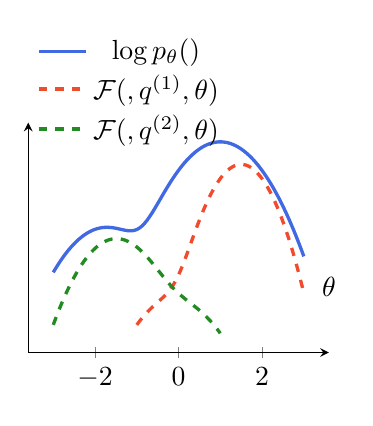
\begin{tikzpicture}
  % Plot settings
  \begin{axis}[
    xlabel=$\theta$, 
    % ylabel={Log likelihood}, 
    axis lines=left, 
    enlargelimits, 
    height=4.5cm, 
    width=5.4cm,
    % legend pos=north west + (0, -0.5cm),
    % legend pos=south,
    yticklabels={},
    ytick=\empty,   % Remove y-axis ticks
    xlabel style={at={(axis description cs:1.0,+0.2)},anchor=south},
    legend style={at={(0,.86)}, anchor=south west, draw=none, fill=none},
    % title={Variational Lower Bound Visualization}
  ]
    
    % True log likelihood (log p(x|theta))
      \addplot[domain=-3:3, samples=100, very thick, RoyalBlue] {ln(2*exp(-(x-1)^2) + 0.1*exp(-(x+1.75)^2))};
    \addlegendentry{$\log p_{\theta}(\rvx)$}

    % Variational lower bound option 1
    \addplot[domain=-1:3., samples=100, very thick, RedOrange, dashed] {ln( 100 * exp(-(x-1.5)^2/0.5) + exp(-(x)^2)) - 4.7};
    \addlegendentry{$\mathcal{F}(\rvx, q^{(1)}, \theta)$}
    % Variational lower bound option 2
    \addplot[domain=-3:1, samples=100, very thick, ForestGreen, dashed] {ln( 10 * exp(-(x+1.5)^2/0.75) + exp(-(x)^2)) - 5.};
    \addlegendentry{$\mathcal{F}(\rvx, q^{(2)}, \theta)$}
  \end{axis}
\end{tikzpicture}
\caption{Illustration of the log likelihood (solid line) and two variational lower bounds (dashed lines) corresponding to different variational distributions $q$.}\label{fig:intro_bound}
\end{marginfigure}

To see how ELBO relates to maximum likelihood and posterior approximation,  consider the following decomposition:
\begin{equation}
\begin{aligned}
    \mathcal{F}(\rvx, q, \theta) &= \E_{q(\rvz)}\log  \frac{p_{\theta}(\rvx,\rvz)}{q(\rvz)} \\
    & = \E_{q(\rvz)}\log  \frac{p_{\theta}(\rvz|\rvx)p_{\theta}(\rvx)}{q(\rvz)} \\
    & = \E_{q(\rvz)}\log  \frac{p_{\theta}(\rvz|\rvx)}{q(\rvz)} +  \log p_{\theta}(\rvx)\\
    & = - \KL{q(\rvz)}{p_{\theta}(\rvz|\rvx)} + \log p_{\theta}(\rvx).\\
\end{aligned}
\end{equation}
This shows that ELBO is equal to the sum of marginal likelihood and the negative KL divergence between the introduced distribution $q(\rvz)$ and the true posterior.
% and makes it clear that the bound is tight when $q(\rvz) = p(\rvz|\rvx)$. 
Thus,  maximizing ELBO with respect to the distribution $q$ is identical to minimizing this KL divergence. When $q(\rvz) = p(\rvz|\rvx)$ the divergence is zero and the ELBO matches the log likelihood.
Moreover, \citet{neal1998view} showed that if $\mathcal{F}(\rvx, q, \theta) $ has a maximum at $q^*, \, \theta^*$, then $\log p_{\theta}(\rvx)$ has a maximum at $\theta^*$. That is, ELBO has the same optimum as the maximum likelihood objective. 

\paragraph{Expectation Maximization}
Expectation Maximization Algorithm~\citep{dempster1977maximum} (EM-algorithm for short) is an iterative algorithm to infer posterior over the latent variables and the maximum likelihood estimate of the parameters.
It is usually applied to a class of problems, where $p_{\theta}(\rvz|\rvx)$ is tractable if we fix parameters of the generative model $\theta$. Each iteration consists of \textit{expectation step} (E-step) and \textit{maximization step} (M-step) defined below.
\begin{equation}
\begin{aligned}
    \text{\textbf{E-step:  }} &q^{t+1}_n(\rvz) = p_{\theta^t}(\rvz|\rvx_n) = \arg\max_{q_n} \mathcal{F}(\rvx_n, q_n, \theta^t),\;\;\forall n \in \{1\dots N\};\\
    \text{\textbf{M-step:  }} &\theta^{t+1} = \arg\max_{\theta} \E_{p_e(\rvx)}\mathcal{F}(\rvx, q^{t+1}_n, \theta).\\
\end{aligned}
\end{equation}
The expectation step computes the posterior distribution given the model parameters from the previous step. Maximization step uses this posterior to optimize the ELBO with respect to parameters $\theta$. From the formulation above, we also see that both steps of the EM-algorithm solve the same optimization problem: maximizing the ELBO.  This observation allows us to generalize this to a wider class of problems where the posterior distribution is not tractable. 

\paragraph{Variational Inference}
% When EM-algorithm is intractable, one can still use ELBO as a training objective. 
As we said before, Variational Inference essentially turns the posterior inference problem into the optimization problem.
Assume that $q_n$,  variational posterior distribution for a datapoint $\rvx_n$ belongs to a parametric family of distributions defined by parameters $\phi_n$:
\begin{equation}
    \mathcal{Q} = \{q_{\phi_n}(\rvz) | \phi_n \in \Phi\}.
\end{equation}
Note that we assume that each of $q_{\phi_n}(\rvz)$ is independent of each other, which is known as a \textit{mean-field assumption}. We call $\phi_n$ local parameters, since they are learned separately for each datapoint, as opposed to global parameters $\theta$. The resulting objective is: 
\begin{equation}
     \mathcal{L}^{VI}(\rvx_n, \phi_n, \theta) =  \E_{q_{\phi_n}(\rvz)}\log  \frac{p_{\theta}(\rvx_n|\rvz)p_{\theta}(\rvz)}{q_{\phi_n}(\rvz)}.
\end{equation}
\begin{marginfigure}
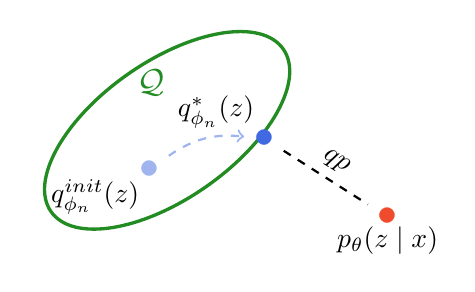
\begin{tikzpicture}
    % Draw the circle representing the variational family
    \draw[very thick, ForestGreen, rotate=35] (0,0) ellipse (1.8cm and 0.87cm) node[above, yshift=0.3cm, xshift=-0.2cm]  {\large$\mathcal{Q}$};
    
    % Point for the true posterior outside the circle
    \node[RedOrange] (trueposterior) at (2.8, -1.1) {\Large$\bullet$};
    \node[below] at (trueposterior) {\normalsize$ p_{\theta}(z \mid x) $};
    
    % Point for the variational distribution on the border of the circle
    \node[RoyalBlue!50] (varfamily_init) at (-0.23, -.5) {\Large$\bullet$};
    \node[below left] at (varfamily_init) {\normalsize $q^{\text{init}}_{\phi_n}(z) $};
    
    \node[RoyalBlue] (varfamily) at (1.23, -.1) {\Large$\bullet$};
    \node[above left] at (varfamily) {\normalsize $q^*_{\phi_n}(z) $};

     % Curvy line between varfamily_init and varfamily
    \draw[thick, RoyalBlue!50, ->, dashed, bend left=20] (varfamily_init) to (varfamily);
    
    % Arrow from variational family to true posterior
    \draw[-, dashed, thick] (varfamily) -- (trueposterior) node[midway, above, sloped] {$\KL{q}{p}$};
\end{tikzpicture}
\caption{When posterior distribution $ p_{\theta}(z \mid x) $ lies outside of variational family $\mathcal{Q}$, variational inference seeks to find the approximation $q^*_{\phi_n}(z) $ which is closest to the true posterior in terms on KL divergence} \label{fig:intro_vi}
\end{marginfigure}
Optimizing this objective function yields $q_{\phi_n}$ from a chosen family of distributions, which is closest to the true posterior in terms of KL divergence (see Figure~\ref{fig:intro_vi} for illustration). Similarly to the stochastic version of the gradient descent, stochastic Variational Inference (SVI) was proposed~\citep{hoffman2013stochastic}, where at each iteration only a subset of data is used and thus only a subset of local variational parameters $\phi_n$ is updated. 
However, there are still multiple aspects that hinder the scalability of the VI objective. We will now address each of these in detail. 


\paragraph{Amortized Variational Inference}
Having separate local parameters for each data point can be very expensive. 
A common way to overcome it is to use amortization. This approach restricts the family of variational distributions even further, assuming that each of the $q_n$'s is parametrized with the same Neural Network $f_{\phi}$, which maps a datapoint $\rvx_n$ to the corresponding parameters of the distribution: 
\begin{equation}
    % \mathcal{Q}_{\text{A}} = \Big\{ q: \prod_n q_{\phi}(\rvz | \rvx_n) \Big\}
    q_{\phi_n}(\rvz) = q_{\phi}(\rvz |\rvx_n).
\end{equation}
The amortized family is a subset of the mean-field variational family and the difference in the quality of the resulting approximations is known as \textit{Amortization Gap}~\citep{cremer2018inference}. It was also shown that a middle ground between AVI and SVI achieves better performance~\citep{kim2018semi}. However, on a large scale, even a small computational overhead can be detrimental. Therefore, throughout this thesis, we will use amortized variational inference objective:
\begin{equation}\label{eq:intro_avi}
     \mathcal{L}^{AVI}(\rvx, \phi, \theta) =  \E_{q_{\phi}(\rvz)}\log  \frac{p_{\theta}(\rvx|\rvz)p_{\theta}(\rvz)}{q_{\phi}(\rvz|\rvx)}.
\end{equation}

\paragraph{Reparametrization trick and doubly stochastic variational inference}
Finally, in order to learn both the generative parameters $\theta$ and the variational parameters $\phi$, we need an efficient way to compute the gradients. 
Assume first that the parametric form of $p_{\theta}(\rvx|\rvz)$, $p_{\theta}(\rvz)$ and $q_{\phi}(\rvz|\rvx)$ allows us to compute the corresponding gradients $\nabla_{\theta}\log p_{\theta}(\rvx|\rvz)$, $\nabla_{\theta}\log p_{\theta}(\rvz)$, and $\nabla_{\theta}\log q_{\phi}(\rvz|\rvx)$ using backpropagation. 
Then the gradient of the evidence lower bound w.r.t. $\theta$ is straightforward to calculate.
\begin{equation}\label{eq:avi_grad_theta}
    \begin{aligned}
      \nabla_{\theta}\mathcal{L}^{AVI}(\rvx, \phi, \theta) 
      &= \E_{q_{\phi}(\rvz|\rvx)} \nabla_{\theta} \log  \frac{p_{\theta}(\rvx|\rvz)p_{\theta}(\rvz)}{q_{\phi}(\rvz)} \\
      &= \E_{q_{\phi}(\rvz|\rvx)} \nabla_{\theta} \log p_{\theta}(\rvx|\rvz)p_{\theta}(\rvz).
    \end{aligned}
\end{equation}
This quantity can be efficiently computed using Monte Carlo estimation. In practice, even one-sample estimation works well:
\begin{equation}
\begin{aligned}
    \nabla_{\theta}\mathcal{L}^{AVI}(\rvx, \phi, \theta) &\approx \nabla_{\theta} \log p_{\theta}(\rvx|\tilde{\rvz})p_{\theta}(\tilde{\rvz}),\\
    \tilde{\rvz} &\sim q_{\phi}(\rvz|\rvx).
    \end{aligned}
\end{equation}
However, since the expectation in Eq.~\ref{eq:intro_avi} is taken with respect to $q_{\phi}(\rvz|\rvz)$, computing the gradient with respect to the parameters of the variational distribution is less straightforward.
It can be computed using the method called REINFORCE~\citep{williams1992simple} or with the help of the reparameterization trick. 

REINFORCE uses the log-derivative trick to convert the gradient of the expectation into the expectation of the gradient, of the form similar to Eq.~\ref{eq:avi_grad_theta}. 
However, it tends to have a high variance and is not often used in generative modeling. 
\marginnote[-3\baselineskip]{Log derivative uses the definition of the gradient of the logarithm which gives: $$\nabla_{\phi}q_{\phi}(\rvz) = q_{\phi}(\rvz)\nabla_{\phi}\log q_{\phi}(\rvz)$$.}

A more commonly used method, the reparameterization trick, was independently proposed for latent variable generative models~\cite{kingma2014autoencoding, rezende2014stochastic} and for Bayesian inference~\citep{titsias2014doubly}. 
Consider a random variable $\varepsilon \sim p(\varepsilon)$ and a deterministic transformation $g_{\phi}(\varepsilon, \rvx)$, such that:
\begin{equation}
    \tilde{\rvz} = g_{\phi}(\varepsilon, \rvx)\quad \Rightarrow \quad  \tilde{\rvz} \sim q_{\phi}(\rvz|\rvx).
\end{equation}
We can now use this deterministic transformation to apply change of variable formula to the Eq.~\ref{eq:intro_avi}:
\begin{equation}
\begin{aligned}
     \mathcal{L}^{AVI}(\rvx, \phi, \theta) &=  \E_{p(\varepsilon)}\log  \frac{p_{\theta}(\rvx|\tilde{\rvz})p_{\theta}(\tilde{\rvz})}{q_{\phi}(\tilde{\rvz}|\rvx)},\\
     \text{where}\; \tilde{\rvz} &= g_{\phi}(\varepsilon, \rvx).
\end{aligned}
\end{equation}
In this way, we move all trainable parameters inside the expectation, and the Monte Carlo estimate of the gradient with respect to $\phi$ can be easily computed. 
\begin{equation}
\begin{aligned}
    \nabla_{\phi}\mathcal{L}^{AVI}(\rvx, \phi, \theta) &\approx  \nabla_{\phi}\log  \frac{p_{\theta}(\rvx|\tilde{\rvz})p_{\theta}(\tilde{\rvz})}{q_{\phi}(\tilde{\rvz}|\rvx)}, \\
    \text{where}\quad \tilde{\rvz} &= g_{\phi}(\tilde{\varepsilon}, \rvx)\,\text{ and }\, \tilde{\varepsilon} \sim p(\varepsilon).
\end{aligned}
\end{equation}
Note that with this approach, we have two sources of stochasticity. 
At each training step, we use a subsample of the data points (a mini-batch) $\{\rvx_i\}_{i \in \mathcal{M}}$ to estimate the expectation with respect to the empirical distribution $p_{e}(\rvx)$, and we sample the latent variable (by the mean of the Reparameterization trick) to estimate the expectation with respect to the variational distribution $q_{\phi}(\rvz|\rvx)$. 
For this reason, \citet{titsias2014doubly} referred to such method as \textit{Doubly Stochastic Variational Inference} (DDVI). 
However, this term is more common in Bayesian inference rather than in Deep Generative Modeling. 
Therefore, throughout this thesis, we will mostly refer to it as Amortized Variational Inference with Reparametrization trick.


%%%%%%%%%%%%%%%%%%%%%%%%%%%%%%%%%5
% Auxiliarly variables: latent and non-latent
%%%%%%%%%%%%%%%%%%%%%%%%%%%%%%%%%5
\section{Latent Variable Models}\label{sec:into_latent_variable_models}
%- Latent variable generative models: from PPCA to Diffusion models
%- $$p(x) = p(x|z)p(z)$$
%- Lower dimentional manifold assumption
%- Oldies but goldies: PPCA -> Helmholtz machines / Boltzman machines 
%- Modern heros: Variational Autoencoders, Diffusion Models
%- Amortization and voila, we have variational posterior $$q(z|x)$$
This thesis contributes to the field of Variational Autoencoders (VAEs) and Diffusion Models. These are deep generative models with latent variables and are trained with the Amortized Variational Inference discussed above. We will now discuss both of these models in more detail.
% We consider the application of these models to the problem of modeling the distribution of images in different scenarios. 

\subsection{Variational Autoencoder}
Variational Autoencoder is the first generative model that we will consider. 
First, let us take a closer look at the Evidence Lower Bound (Eq.~\ref{eq:intro_avi}) that is used to train VAEs. There are multiple ways to rewrite this objective which give rise to different intuitions regarding the model. We start from the following decomposition:
\begin{equation}\label{eq:intro_elbo_again}
\mathcal{L}(\theta, \phi) = \E_{p_e(\rvx)}\Big[ \underbrace{\E_{q_{\phi}(\rvz|\rvx)} \log p_{\theta}(\rvx| \rvz)}_{\text{Reconstruction}} - \underbrace{\KL{q_{\phi}(\rvz|\rvx)}{p_{\theta}(\rvz)}}_{\text{KL term}} \Big].
\end{equation}
% This generative model can be interpreted as an infinite mixture model \cite{mattei2018leveraging}. 
% Here \cite{mattei2018leveraging}, this interpretation allowed to obtain an upper bound on the likelihood. 
\paragraph{Reconstruction}
\marginnote[4\baselineskip]{Variational posterior $q_{\phi}(\rvz|\rvx)$ is commonly called \textit{encoder} and the conditional likelihood $p_{\theta}(\rvx|\rvz)$ \textit{decoder}. Thus, when both distributions are learned together, the resulting model can be seen as a probabilistic \textit{autoencoder}, hence the model's name.} 
The first part of the ELBO in Eq.~\ref{eq:intro_elbo_again} ensures that the model is able to reconstruct the input $\rvx$. If we consider it's Monte Carlo estimator for a single datapoint, it is computed by first sampling $\tilde{\rvz}_n$ for a given datapoint from the variational posterior
and then computing the conditional log-likelihood using this sample:
\begin{align}
    \tilde{\rvz}_n &\sim q_{\phi}(\cdot|\rvx_n), \label{eq:intro_encode}\\
    \text{Re}(\rvx_n) &= \log p_{\theta}(\rvx_n|\tilde{\rvz}_n).\label{eq:intro_decode}
\end{align}
In other words, we \textit{encode} data into the latent space in Eq.~\ref{eq:intro_encode} and then \textit{reconstruct} it (or in other words get parameters of the conditional likelihood given the latent variable) to compute the reconstruction term in Eq.~\ref{eq:intro_decode}.

\paragraph{KL term}
The second term in Eq.~\ref{eq:intro_elbo_again} can be seen as a regularizer. It ensures that the variational posterior is close to the distribution $p_{\theta}(\rvz)$, which is usually called \textit{prior}.
Thus, after training a model, one can sample latent code from the prior \textit{unconditionally} and then decode it using the conditional likelihood. 
\marginnote[-4\baselineskip]{
The name \textit{prior} often suggests that this distribution is given to us \textit{apriori}. However, we will often employ an approach in which the distribution $p_{\theta}(\rvz)$ has learnable parameters and is learned together with the conditional likelihood. This is analogous to the empirical Bayes \cite{wang2019comment} approach, where prior is estimated from the data. 
}

\paragraph{Constrained Optimization Framework}
One can also consider the objective ELBO from the constrained optimization point of view \citep{higgins2017beta, rezende2018taming}. \citet{higgins2017beta} introduce $\beta$-VAE, where additional hyperparameter $\beta$ is used to re-weight the KL-term in Eq.~\ref{eq:intro_elbo_again}. \citet{rezende2018taming} introduce Generalized ELBO with Constrained Optimization, where they treat the VAE objective as the minimization of the KL divergence subject to the reconstruction constraint. The Lagrangian for this problem becomes ELBO with the additional parameters $\lambda$ (the Lagrange multiplier). They propose using the moving average of the constraint to update the Lagrange multiplier.
\citet{klushyn2019learning} proposes a different rule for updating $\lambda$, which ensures that the model optimizes ELBO once the reconstruction constraint is met. 

\paragraph{Approximating Likelihood with Importance Sampling}
As we have already mentioned, estimating the likelihood exactly is difficult for the latent variable model, due to the intractability of the integral. However, we can still approximate it using important sampling (IS). For each datapoint $\rvx$, we use the variational posterior distribution as a proposal. IS likelihood estimate is obtained by sampling $K$ times from the proposal and computing the weighted average:
\begin{equation}
\begin{aligned}
    \log p_{\theta}(\rvx) = \int p_{\theta}(\rvx|\rvz)p_{\theta}(\rvz)d\rvz \approx &\log \frac1K \sum_k\frac{p_{\theta}(\rvx|\tilde{z}_k)p_{\theta}(\tilde{z}_k)}{q_{\phi}(\tilde{z}_k|\rvx)},\\
    &\tilde{z}_k \sim q_{\phi}(\rvz|\rvx).
\end{aligned}
\end{equation}
This is known as an \textit{importance weighted} log likelihood estimate. Notice that for $K=1$ it is equal to the ELBO. Furthermore, as we increase $K$ the bound on the log likelihood becomes tighter, and it approaches $\log p_{\theta}(\rvx)$ as $K \rightarrow \infty$~\citep{burda2015importance}. In practice $K=500$ or $K=1000$ is commonly used to report the test log-likelihood results and to compare the performance of different models. \citet{burda2015importance} proposed to use this as a training objective, a model known as \textit{Importance Weighted Autoencoder} (IWAE). 

\paragraph{Model Components}
Latent Variable model, including a VAE, consists of three main components. The conditional likelihood $p_{\theta}(\rvx|\rvz)$, which models the distribution of the data given its latent representation. The prior $p_{\theta}(\rvz)$, which is the marginal distribution over the latent space. And finally, the variational posterior $q_{\phi}(\rvz|\rvx)$, which models a conditional distribution of the latent variable given the data. We will now discuss each of these three components.
% \paragraph{Information Theoretic Point of View}
% \addpart{fixing the broken ELBO}
% Auxiliary Deep Generative Models \cite{maaloe2016auxiliary}
% \paragraph{VAE limitations}
% \begin{itemize}
%     \item Blurry samples \cite{Rybkin2020-je}
%     \item Posterior Collapse \\
%     \cite{kingma2016improved} proposed free bits to solve posterior collapse    
%     \item Holes in the latent space\\
%     A more flexible prior to cover the aggregated posterior better
% \end{itemize}

\subsection{Conditional Likelihood}
The choice of conditional likelihood is usually determined by the type of data. For example, we may use the Gaussian distribution for continuous data with infinite support. Another common option is the Bernoulli distribution for discrete binary-valued data. 

\paragraph{Modeling pixel values}
In this thesis we mainly conduct experiments in the computer vision domain, modeling distribution of images.
Each pixel of an image can be seen as a continuous random variable representing the intensity $\nu$. 
However, the observed value $\rvx$ is usually discretized (e.g. intensity rounded to the nearest 8-bit representation). 
Therefore, using a continuous distribution might be suboptimal.
An option in this case would be to use the categorical distribution with 256 possible values for each pixel (in the case of the 8-bit representation). However, this will ignore the fact that the nearby pixel values are correlated. 
Instead, a common approach is to model the pixel intensity as a continuous random variable and then discretize its distribution to calculate the actual likelihood. 


We will assume that all pixels across spacial and channel dimensions are conditionally independent:
\begin{align}
    p_{\theta}(\rvx|\rvz) &= \prod_i p_{\theta}(\rvx_i|\rvz),\\
    p_{\theta}(\rvx_i|\rvz) &= \sum_{k} P_{\theta}(\rvx_i = k|\rvz).
\end{align}
Here $\rvx_i$ is a single pixel of an image in an 8-bit representation and $k$ is a particular pixel value. 
Assume that the intensity of the pixels has a continuous distribution with the probability density function $f_{\nu}$ and the cumulative distribution function (CDF) $F_{\nu}$. We can discretize it in two ways. 

The first option is to split the support of the intensity random variable into bins and compute probability of each bin via integration:
\begin{equation}\label{eq:intro_int_discr}
\begin{aligned}
    &P_{\theta}(\rvx_i = k|\rvz) = \int_{\delta_{-}(\rvx_i)}^{\delta_{+}(\rvx_i)} f_{\nu}(\nu|\rvz)d\nu,\\
    &\delta_{-}(\rvx_i) =
    \begin{cases}
        \infty,\quad &\text{if } \rvx_i = 0\\
        \rvx_i + \frac12,\quad&\text{otherwise}
    \end{cases};  \quad
    \delta_{+}(\rvx_i) =
    \begin{cases}
        -\infty,\quad &\text{if } \rvx_i = 255\\
        \rvx_i - \frac12,\quad&\text{otherwise}
    \end{cases}.
\end{aligned}
\end{equation}
Assuming that we know the CDF of the intensity, we can compute the value of the integral as follows:
\begin{equation}
    P_{\theta}(\rvx_i = k|\rvz) =\begin{cases}
    F_{\nu}(\rvx_i + \frac{1}{2}) - F_{\nu}(\rvx_i - \frac{1}{2}),\quad &\text{if } k \in (1, \dots, 254) \\
    F_{\nu}(\rvx_i + \frac{1}{2}) - 0,\quad &\text{if } k = 0 \\
    1 - F_{\nu}(\rvx_i - \frac{1}{2}),\quad &\text{if } k = 255 \\
    \end{cases}.
\end{equation}
It is convenient to use logistic distribution~\cite{kingma2016improved}, as it's CDF can be easily computed:
\begin{equation}
    F^{\text{logistic}}(x; \mu, \sigma) = \frac{1}{1 + \exp (- \frac{x - \mu}{\sigma})}.
\end{equation}
\begin{marginfigure}
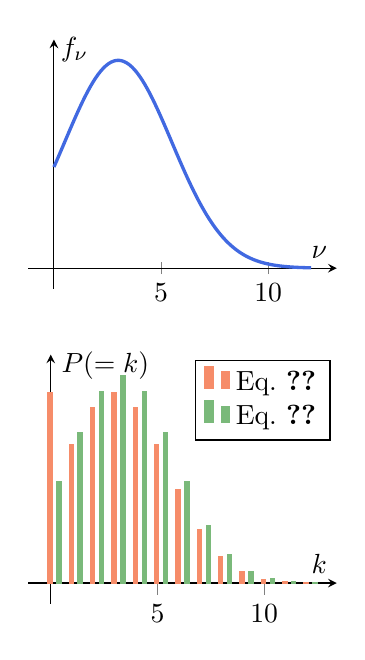
\begin{tikzpicture}
  \begin{axis}[
  name=plot1,
    domain=0:12, 
    samples=100, 
    xlabel=\normalsize$\nu$, 
    ylabel=\normalsize$f_{\nu}$, 
    axis lines=middle, 
    enlargelimits, 
    % title={Intensity}, 
    % height=4cm, 
    width=5.5cm,
    yticklabels={},
    ytick=\empty,   % Remove y-axis ticks
    ylabel style={at={(axis description cs:+0.15,1.05)},anchor=north},
  ]
    \addplot[very thick, RoyalBlue] {1/(sqrt(2*pi*6.25)) *  exp(-0.5 * (x-3)^2/6.25};
  \end{axis}

  \begin{axis}[
  name=plot2,
  at={(0,-4cm)},
    % domain=0:15, 
    % samples=100, 
    xlabel=\normalsize $ k $, 
    ylabel={\normalsize$ P(\rvx=k)$}, 
    axis lines=middle, 
    enlargelimits, 
    % title={Pixel Values}, 
    % height=4cm, 
    width=5.5cm,
    ybar,
    bar width=0.2,
    yticklabels={},
    ytick=\empty,   % Remove y-axis ticks
    ylabel style={at={(axis description cs:+0.25,1.05)},anchor=north},
  ]
   % Discrete points from the Gaussian distribution
    \addplot[RedOrange!60, fill=RedOrange!60] coordinates {
(0.2, 0.1588)
(1.2, 0.1155)
(2.2, 0.1464)
(3.2, 0.1585)
(4.2, 0.1464)
(5.2, 0.1155)
(6.2, 0.0779)
(7.2, 0.0450)
(8.2, 0.0222)
(9.2, 0.0093)
(10.2, 0.0033)
(11.2, 0.0009)
(12.2, 0.0002)
    };
     \addlegendentry{Eq.~\ref{eq:intro_int_discr}}
    % Discrete points from the Gaussian distribution
    \addplot[ForestGreen!60, fill=ForestGreen!60] coordinates {
(0.15, 0.0844)
(1.15, 0.1259)
(2.15, 0.1600)
(3.15, 0.1733)
(4.15, 0.1600)
(5.15, 0.1259)
(6.15, 0.0844)
(7.15, 0.0482)
(8.15, 0.0235)
(9.15, 0.0097)
(10.15, 0.0034)
(11.15, 0.0010)
(12.15, 0.0003)
    };
    \addlegendentry{Eq.~\ref{eq:intro_softmax_discr}}
    % \addplot[blue, thick] {1/(sqrt(2*pi*0.5)) *  exp(-0.5 * (x-5)^2/0.5};
  \end{axis}
    % Arrow from the first plot to the second plot
  % \draw[->, thick](plot1.south east) -- (plot2.north west) node[midway, right] {};

\end{tikzpicture}
\caption{Probability Density Function for the pixel intensity (top) and discretized probabilities (bottom)}
\end{marginfigure}
\citet{salimans2016improved} proposed to use a mixture of discretized logistic distributions to improve the flexibility of the distribution.

The second option is to re-normalize the probability of each bin:
\begin{equation}\label{eq:intro_softmax_discr}
\begin{aligned}
    P_{\theta}(\rvx_i = k|\rvz) = \frac{f_{\nu}(k|\rvz)}{\sum_{i=0}^K f_{\nu}(i|\rvz)}.
\end{aligned}
\end{equation}
Note that in this case, we only need to know the PDF of the pixel intensity up to a normalization constant. 
Thus, it is convenient when we want to use the Gaussian distribution:
\begin{equation}
\begin{aligned}
    P_{\theta}(\rvx_i = k|\rvz) = \frac{\exp\left(-\frac12 \left(\frac{\mu_{\theta}(\rvz) - k}{\sigma_{\theta}(\rvz)}\right)^2\right)}{\sum_{i=0}^{255} \exp\left(-\frac12 \left(\frac{\mu_{\theta}(\rvz) - i}{\sigma_{\theta}(\rvz)}\right)^2\right)}.
\end{aligned}
\end{equation}
There is one more difference between the two approaches. The first tends to assign a higher probability to the pixel values 0 and 255. \citet{salimans2016improved} motivated this by the observation that these values have a higher frequency in real data. Renormalization, on the other hand, divides all bins by the same normalization constant. This is illustrated in Figure~\ref{eq:intro_int_discr}.
In practice, both discretizations are used. 
For example, logistic distribution~\citep{vahdat2020nvae, Child2020-ze} discretized with CDF, Gaussian distribution~\citep{ho2020denoising} discretized with CDF, and renormalized Gaussian distribution~\citep{kingma2021variational}. 
In our experiments, we found all three options to perform similarly. 

\subsection{Learnable Prior}
Another important component of the latent variable generative models is the prior over the latent variables $p_{\theta}(\rvz)$.
It can be used to impose structure or specific inductive biases. 
Early VAE works used the most uninformative version of the prior, an isotropic Gaussian with zero mean.
\begin{equation}
    p(\rvz) = \mathcal{N}(\rvz | 0, \text{I}).
\end{equation}
\marginnote[-2\baselineskip]{Note that this way prior does not have any trainable parameters; therefore, the $\theta$ subscript is removed.}\newline
However, this prior can be too restrictive and can cause a problem known in the VAE literature as \textit{holes} in the latent space. Intuitively, we can think of a hole as regions in the latent space with high prior probability, which is not covered by any of the variational posterior distributions. 

To better understand the problem of holes in the latent space, consider a toy example with the 2-dimensional latent space in Figure~\ref{fig:intro_prior_mismatch}. 
The top plot depicts a standard Gaussian prior and the darkness of the color represents the probability of the sample. 
Let us also define the \textit{aggregated posterior} as a variational posterior averaged over the entire dataset: $q_{\phi}(\rvz) = \E_{p_{e}(\rvx)}q_{\phi}(\rvz|\rvx)$. 
The bottom plot of Figure~\ref{fig:intro_prior_mismatch} presents a mixture of Gaussian distributions that is spread around the same area of the 2-d plane as the prior above it. 
However, there are several places where the aggregated posterior has a very low probability, namely, no real data point $\rvx$ is ever encoded in this part of the latent space. 
At the same time, the prior distribution assigns a high probability to this region. One such area is denoted by a red circle in the figure. 
This motivates the use of more complicated prior distributions, which are capable of \textit{adapting} to the aggregated posterior and are flexible enough to avoid holes. 
\begin{marginfigure}
\vspace*{-10\baselineskip}
\subfloat[Prior \label{subfig:intro_prior}]{
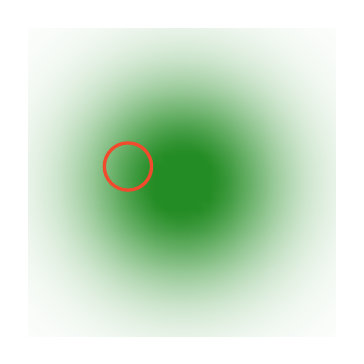
\begin{tikzpicture}
\begin{axis}[
    width=5.5cm,
    height=5.5cm,
    axis lines=none,
    colormap={greenmap}{color(0cm)=(ForestGreen!1); color(1cm)=(ForestGreen!99)},
    point meta min=0, point meta max=1,
    view={0}{90}
]
\addplot3[
    surf,
    shader=interp,
    samples=30,
    domain=-2:2,
    domain y=-2:2
]{exp(-0.5*(x^2 + y^2) / 0.9^2) / 0.9};
\draw[very thick, RedOrange] (-0.7,0.2) circle (0.3cm); 
\end{axis}
\end{tikzpicture}
}
\vskip 5pt
\subfloat[Aggregated Posterior \label{subfig:intro_agg_posterior}]{
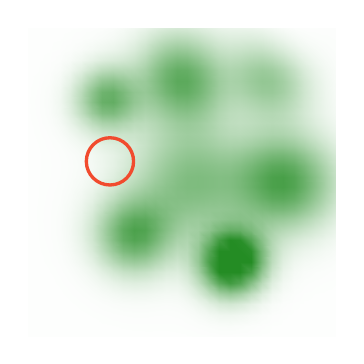
\begin{tikzpicture}
\begin{axis}[
    width=5.5cm,
    height=5.5cm,
    axis lines=none,
    colormap={greenmap}{color(0cm)=(ForestGreen!1); color(1cm)=(ForestGreen!99)},
    point meta min=0, point meta max=1,
    view={0}{90}
]
\addplot3[
    surf,
    shader=interp,
    samples=30,
    domain=-1.5:1.5,
    domain y=-1.5:1.5
]
{
(1/6 * exp(-0.5*((x-1)^2 + y^2) / 0.35^2) / 0.35 
+ 1/6 * exp(-0.5*(x^2 + (y-1)^2) / 0.3^2) / 0.3 
+ 1/6 * exp(-0.5*((x-0.9)^2 + (y-1.1)^2) / 0.28^2) / 0.28 
+ 1/6 * exp(-0.5*((x)^2 + y^2) / 0.4^2) / 0.4 
+ 1/6 * exp(-0.5*((x-0.5)^2 + (y+0.8)^2) / 0.21^2) / 0.15
+ 1/6 * exp(-0.5*((x+0.75)^2 + (y-0.8)^2) / 0.21^2) / 0.25
+ 1/6 * exp(-0.5*((x+0.5)^2 + (y+0.5)^2) / 0.25^2) / 0.25 ) * (0.8 + 0.4*sin(100*x)*cos(100*y) + 0.5*cos(90*x*y))
};
\draw[very thick, RedOrange] (-0.7,0.2) circle (0.3cm); 
\end{axis}
\end{tikzpicture}
}
\caption{Example of the mismatch between the prior (top plot) and aggregated posterior (bottom)}\label{fig:intro_prior_mismatch}
\end{marginfigure}

A flexible prior with trainable parameters can be viewed as a generative model in itself. 
Note that we need to choose a model with fully tractable likelihood to ensure the tractability of the ELBO.
For example, \citet{chen2016variational} proposed to employ Autoregressive Normalizing Flows as a learnable prior in the VAEs. This class of models employs a change-of-variable formula to compute the model density, as we discussed in Section~\ref{subsec:intro_gen_zoo}. 

Even with a highly flexible prior, the question remains which prior is optimal with respect to ELBO maximization.
To answer this question, we will follow \citet{hoffman2016elbo} and decompose the KL-term of the ELBO into two components.
\begin{align}
&\KL{q_{\phi}(\rvz|\rvx)}{p_{\theta}(\rvz)} = \int q_{\phi}(\rvz|\rvx) \log \frac{q_{\phi}(\rvz|\rvx)}{p_{\theta}(\rvz)}\frac{q_{\phi}(\rvz)}{q_{\phi}(\rvz)}d\rvz \label{eq:elbo_prior_1}\\
 &\quad=\int q_{\phi}(\rvz|\rvx) \log \frac{q_{\phi}(\rvz)}{p_{\theta}(\rvz)}d\rvz  + \int  q_{\phi}(\rvz|\rvx) \log \frac{q_{\phi}(\rvz|\rvx)}{q_{\phi}(\rvz)}d\rvz   \label{eq:elbo_prior_2} \\
 &\quad=\int q_{\phi}(\rvz|\rvx) \log \frac{q_{\phi}(\rvz)}{p_{\theta}(\rvz)}d\rvz  + \int  q_{\phi}(\rvz|\rvx) \log \frac{q_{\phi}(\rvz, \rvx)}{q_{\phi}(\rvz) p_e(\rvx)}d\rvz.  \label{eq:elbo_prior_3}
\end{align}
\marginnote[-7\baselineskip]{First, we apply the definition of the KL divergence and multiply the integrand by $1$ in Eq.~\ref{eq:elbo_prior_1}. Then, using the logarithm property, we split the equation into two terms in Eq.~\ref{eq:elbo_prior_2}. Finally, we apply Bayes formula in the second term to get Eq.~\ref{eq:elbo_prior_3}.}\newline
Now, we can take an expectation with respect to the data distribution.
\begin{align}\label{eq:intro_kl_to_vamp}
&\E_{p_e(\rvx)} \KL{q_{\phi}(\rvz|\rvx)}{p_{\theta}(\rvz)}  \\
&\quad\quad=\int \underbrace{\E_{p_e(\rvx)} q_{\phi}(\rvz|\rvx)}_{q_{\phi}(\rvz)} \log \frac{q_{\phi}(\rvz)}{p_{\theta}(\rvz)}d\rvz  
+ \iint  \underbrace{q_{\phi}(\rvz|\rvx)p_e(\rvx)}_{q_{\phi}(\rvz, \rvx)} \log \frac{q_{\phi}(\rvz, \rvx)}{q_{\phi}(\rvz) p_e(\rvx)}d\rvz d\rvx \notag\\
&\quad\quad= \KL{q_{\phi}(\rvz)}{p_{\theta}(\rvz)}
+ \text{MI}\left[\rvz; \rvx\right].
\end{align}
\marginnote[-7\baselineskip]{Both terms can be defined as KL divergences. Furthermore, the second one is equal to Mutual Information between observation and latent code, since it is defined as a KL divergence between the joint distribution and a product of marginal distributions: $$\text{MI}\left[\rvx, \rvy \right] = \KL{p(\rvx, \rvy)}{p(\rvx)p(\rvy)}.$$}\newline
Note that the prior distribution is only present in the first term: KL divergence between the aggregated posterior and prior. Therefore, the prior that maximizes the ELBO is equal to the aggregated posterior, the \textit{mixture} of encoders:
\begin{equation}
    p^*(\rvz) = \arg\max_{p(\rvz)}\mathcal{L}(\theta, \phi) = \E_{p_e(\rvx)}q_{\phi}(\rvz|\rvx).
\end{equation}
This decomposition highlights the significance of multimodal priors. 
Motivated by this observation, \citet{tomczak2018vae} proposed VampPrior, a trainable prior for the VAE, defined as a mixture of variational posteriors. 
To avoid overfitting and make the model computationally tractable, this mixture is parameterized by $K$ pseudoinputs instead of the whole training dataset:
\begin{equation}
    p_{\theta}(\rvz) = \frac1K \sum_k q_{\phi}(\rvz|u_k) \approx p_{\theta}^*(\rvz).
\end{equation}
In this case, the pseudoinputs themselves are the trainable part of the prior. In this thesis, we explore how VampPrior can be used to improve density estimation in a dynamic \textit{continual learning} setting. 

Continual learning is a challenging problem of training deep neural networks in an adaptive manner. We assume a sequence of tasks $t=1,\dots,T$ that must be solved by a single model.
The subsets of the data for each task $\train^1, \dots ,\train^T$ arrive sequentially and we have access to only one chunk at a time (e.g. $\train^t$ at time $t$). 
In Figure \ref{fig:intro_cl_plot}, we show this setup schematically for the 3 tasks. 
At each timestamp, we train our model on a new chunk of data (\textcolor{ForestGreen}{Task1}, \textcolor{RoyalBlue}{Task2} and \textcolor{OrangeRed}{Task3}). 
Ultimately, we expect it to generalize well on the data from all three tasks. 
In other words, we expect to obtain a generative model that approximates the distribution covering data from all three tasks.   
\begin{marginfigure}
\vspace*{-4\baselineskip}
\begin{tikzpicture}[>=Stealth, every node/.style={scale=1.0}, line width=1.2pt]
    % Task 1 x=0, label = 1    
    \foreach \y in {-1, 0, 1} {
        \node[circle, draw, fill=white, minimum size=0.3cm] (input0\y) at (-0.25, 0.5*\y+0.5) {};
        \node[circle, draw, fill=ForestGreen!50, minimum size=0.3cm] (output0\y) at (.25, 0.4*\y+0.5) {};
    }
    \foreach \y in {-1, 0, 1} {
        \foreach \z in {-1, 0, 1} {
            \draw[thick] (input0\y) -- (output0\z);
        }
    }
    \node[] (train0) at (0, -.9)  {\normalsize\color{ForestGreen}\(\mathcal{D}^{(1)}_{\text{train}}\)};
    
    % Task 1 x=1.5, label = 2    
    \foreach \y in {-1, 0} {
        \node[circle, draw, fill=white, minimum size=0.3cm] (input1\y) at (1.25, 0.5*\y+0.5) {};
        \node[circle, draw, fill=RoyalBlue!50, minimum size=0.3cm] (output1\y) at (1.75, 0.4*\y+0.5) {};
    }
    \node[circle, draw, fill=white, minimum size=0.3cm] (input11) at (1.25, 0.5*1+0.5) {};
    \node[circle, draw, fill=ForestGreen!50, minimum size=0.3cm] (output11) at (1.75, 0.4*1+0.5) {};
    
    \foreach \y in {-1, 0, 1} {
        \foreach \z in {-1, 0, 1} {
            \draw[thick] (input1\y) -- (output1\z);
        }
    }
    \node[] (train1) at (1.5, -.9)  {\normalsize \color{RoyalBlue}\(\mathcal{D}^{(2)}_{\text{train}}\)};

    % Task 1 x=3, label = 2    
    \node[circle, draw, fill=white, minimum size=0.3cm] (input2-1) at (2.75, -0.5*1+0.5) {};
    \node[circle, draw, fill=RedOrange!50, minimum size=0.3cm] (output2-1) at (3.25, -0.4*1+0.5) {};
    \node[circle, draw, fill=white, minimum size=0.3cm] (input20) at (2.75, 0.5) {};
    \node[circle, draw, fill=RoyalBlue!50, minimum size=0.3cm] (output20) at (3.25, 0.5) {};

    \node[circle, draw, fill=white, minimum size=0.3cm] (input21) at (2.75, 0.5*1+0.5) {};
    \node[circle, draw, fill=ForestGreen!50, minimum size=0.3cm] (output21) at (3.25, 0.4*1+0.5) {};
    \foreach \y in {-1, 0, 1} {
        \foreach \z in {-1, 0, 1} {
            \draw[thick] (input2\y) -- (output2\z);
        }
    }
    \node[] (train2) at (3, -.9)  {\normalsize \color{RedOrange}\(\mathcal{D}^{(3)}_{\text{train}}\)};
    
    % Timeline
    \draw[->, very thick] (-0.5, -1.5) -- (4, -1.5) node[above right] {Time};
    \foreach \x/\label in {0/1, 1.5/2, 3/3} {
        \draw[very thick] (\x, -1.7) -- (\x, -1.3) node[below=0.3cm] {\(\label\)};
    }
\end{tikzpicture}
\caption{Illustration of continual learning framework, where a model is trained on three different tasks sequentially and is expected to generalize on the data from all the tasks.}\label{fig:intro_cl_plot}
\end{marginfigure}
DNNs are known to reduce their quality on previously learned tasks when trained on data from a new one \citep{kirkpatrick2017overcoming}. 
This phenomenon is called \textit{catastrophic forgetting} \citep{mccloskey1989catastrophic} in the literature. 
Since both inference $\Enc{\rvz}{\rvx}$ and generative $\Dec{\rvx}{\rvz}$ models are parameterized by neural networks, the problem is also relevant for VAEs.  

VampPrior is not only a flexible prior distribution, but it also learns a compact representation of the training dataset. 
If the model is well trained, VampPrior approximates the full dataset using $K$ pseudoinputs. 
Furthermore, it is straightforward to expand the expressivity of the mixture distribution by adding a new component.
This motivates the use of this mixture prior in continual learning and raises the first research question.
\rqs{1}
Chapter~\ref{chap:boovae} addresses this research question.
We derive an optimal prior objective for the continual learning setting and propose a greedy algorithm to add components to the mixture when new data is observed. 

\subsection{Hierarchical VAEs}
In the previous section, we discussed the benefits of flexible priors in VAEs.
In this section, we define Hierarchical VAEs, where the prior over the latent space is defined using the product rule of probability, similar to the autoregressive models discussed in Section~\ref{sec:intro_generative_models_types}. 
Let us split the latent space into $L$ groups $\rvz = (\rvz_1, \dots, \rvz_L)$. We assume that the prior distribution has the following autoregressive structure:
\begin{equation}
    p_{\theta}(\rvz) = \prod_{l=1}^L p_{\theta}(\rvz_l|\rvz_{>l}),
\end{equation}
\marginnote[-2\baselineskip]{We denote $\rvz_{<l} = (\rvz_1, \dots, \rvz_{l-1})$ and assume that $\rvz_{<1} = \varnothing$. }\newline
We will call each group of latent variables $\rvz_l$ a \textit{stochastic layer}. This decomposition imposes a structure on the latent space, referred to as a hierarchy. Therefore, the corresponding generative model is called \textit{Hierarchical VAE}. 
With the hierarchical structure in the prior, it is reasonable to assume that the variational posterior has an autoregressive structure as well. We will distinguish BottomUp and TopDown Hierarchical VAEs depending on the order in which it is decomposed. 

\paragraph{BottomUp Inference}
We start with the BottomUp model, where the variational posterior is defined as follows:
\begin{equation}
    q_{\phi}(\rvz|\rvx) = \prod_{l=1}^L q_{\phi}(\rvz_l|\rvz_{<l}, \rvx).
\end{equation}
Figure~\ref{fig:intro_bottom_up_vae} depicts an example of such a model with three stochastic layers.
\begin{marginfigure}
     \begin{tikzpicture}[node distance=.4cm]
    \node[obs, minimum size=0.75cm] (X) {$\rvx$};
  \node[latent, minimum size=0.75cm, above=0.2cm of X] (z1) {$\rvz_1$};
  \node[latent, minimum size=0.75cm, above=0.4cm of z1] (z2) {$\rvz_2$};
  \node[latent, minimum size=0.75cm, above=0.4cm of z2] (z3) {$\rvz_3$};
  \node[inner sep=0,minimum size=0.5cm, above=0.05cm of z3] (k_top) {$q_{\phi}(\rvz|\rvx)$};
  
  \node[inner sep=0,minimum size=0.5cm, left=0.05cm of z1] (k1) {}; % invisible node
  \node[inner sep=0,minimum size=0.5cm, right=0.1cm of X] (k2) {}; % invisible node
  \node[inner sep=0,minimum size=0.5cm, left=0.05cm of z3] (k3) {}; % invisible node
  % ENCODER:ALL ARROWS 
  \draw[-Latex, black] (X) -- (k2.center) |- node[above]{} (z3);
  \draw[-Latex, black] (X) -- (k2.center) |- node[above]{} (z2);
  \draw[-Latex, black] (X) -- (k2.center) |- node[above]{} (z1);
  \draw[-Latex, black] (z1) -- (k1.center) |- node[above]{} (z3);
  \edge[-Latex, black] {z2} {z3};
  \edge[-Latex, black] {z1} {z2};
  \end{tikzpicture}
  % \quad
  \begin{tikzpicture}[node distance=.4cm]
   \node[obs, minimum size=0.75cm] (X_gen) {$\rvx$};
  \node[latent, minimum size=0.75cm, above=0.2cm of X_gen] (z1_gen) {$\rvz_1$};
  \node[latent, minimum size=0.75cm, above=0.4cm of z1_gen] (z2_gen) {$\rvz_2$};
  \node[latent, minimum size=0.75cm, above=0.4cm of z2_gen] (z3_gen) {$\rvz_3$};
  \node[inner sep=0,minimum size=0.5cm, above=0.05cm of z3_gen] (k333) {$p_{\theta}(\rvx, \rvz)$};
  
    \node[inner sep=0,minimum size=0.5cm, left=0.05cm of z3_gen] (k4) {}; % invisible node

    \node[inner sep=0,minimum size=0.5cm, right=0.05cm of z3_gen] (k5) {}; % invisible node
    \node[inner sep=0,minimum size=0.5cm, right=0.05cm of z2_gen] (k6) {}; % invisible node
    \node[inner sep=0,minimum size=0.5cm, right=0.05cm of z1_gen] (k7) {}; % invisible node
    
    % shared path
    \edge[-Latex, black] {z3_gen} {z2_gen};
    \edge[-Latex, black] {z2_gen} {z1_gen};
    \draw[-Latex, black] (z3_gen) -- (k4.center) |- node[above]{} (z1_gen);

    % conditional likelihood
    \draw[-Latex, black] (z3_gen) -- (k5.center) |- (X_gen);
    \draw[-Latex, black] (z2_gen) -- (k6.center) |- (X_gen);
    \draw[-Latex, black] (z1_gen) -- (k7.center) |- (X_gen);
\end{tikzpicture}
\caption{A graphical model for hierarchical VAEs with three stochastic levels and  \textbf{BottomUp} structure.}\label{fig:intro_bottom_up_vae}
\end{marginfigure}
Let us consider the ELBO for this model:
\begin{align}
    \mathcal{L}(\rvx, \theta, \phi) &= \E_{q_{\phi}(\rvz_{1:L}|\rvx)}\log p_{\theta}(\rvx|\rvz_{1:L}) + \E_{q_{\phi}(\rvz_{1:L}|\rvx)} \log \frac{\prod_{l=1}^L q_{\phi}(\rvz_l|\rvz_{<l}, \rvx)}{\prod_{l=1}^L p_{\theta}(\rvz_l|\rvz_{>l})} \label{eq:intro_bottom_up_elbo_1}\\
    &=\E_{q_{\phi}(\rvz_{1:L}|\rvx)}\log p_{\theta}(\rvx|\rvz_{1:L}) +  \sum_{l=1}^L \E_{q_{\phi}(\rvz_{1:L}|\rvx)}\log \frac{ q_{\phi}(\rvz_l|\rvz_{<l}, \rvx)}{p_{\theta}(\rvz_l|\rvz_{>l})}.\label{eq:intro_bottom_up_elbo_2}
\end{align}
Note that the KL term is divided into the sum of $L$ independent terms, each of which has an expectation over all the stochastic layers $(\rvz_1\dots\rvz_L)$. Thus, we need to sample all the latent variables to get a Monte Carlo estimation of each of the terms. This can be inefficient and lead to instabilities during training. 
However, we can overcome this problem by introducing additional constraints. We discuss it in Section~\ref{sec:intro_diffusion}, where we talk about the latent variable perspective on diffusion models. 

\paragraph{TopDown Inference}
\citet{sonderby2016ladder} proposed a different decomposition, which has a more efficient implementation. The idea is to choose the same traversal order in the variational posterior as in the prior:
\begin{equation}
    q_{\phi}(\rvz|\rvx) = \prod_{l=1}^L q_{\phi}(\rvz_l|\rvz_{>l}, \rvx).
\end{equation}
The first advantage of this decomposition is the potential for parameter sharing. 
For instance, consider the example in Figure~\ref{fig:intro_top_down}.
Here, both the prior and the variational posterior for $\rvz_2$ depend on $\rvz_3$, but not on $\rvz_1$. 
Thus, the same neural network can be used in the generative and inference part of the model to extract the features of $\rvz_3$ relevant for the next stochastic layer. 
These shared paths are denoted by \textcolor{RoyalBlue}{blue arrows}.
\begin{marginfigure}
    \begin{tikzpicture}[node distance=.4cm]
  % ENCODER: ALL RV
  \node[obs, minimum size=0.75cm] (X) {$\rvx$};
  \node[latent, minimum size=0.75cm, above=0.2cm of X] (z1) {$\rvz_1$};
  \node[latent, minimum size=0.75cm, above=0.4cm of z1] (z2) {$\rvz_2$};
  \node[latent, minimum size=0.75cm, above=0.4cm of z2] (z3) {$\rvz_3$};
  \node[inner sep=0,minimum size=0.5cm, above=0.05cm of z3] (k_top) {$q_{\phi}(\rvz|\rvx)$};
  
  \node[inner sep=0,minimum size=0.5cm, right=0.1cm of X] (k2) {}; % invisible node
  \node[inner sep=0,minimum size=0.5cm, left=0.05cm of z3] (k3) {}; % invisible node
  % ENCODER:ALL ARROWS 
  \draw[-Latex, black] (X) -- (k2.center) |- node[above]{} (z3);
  \draw[-Latex, black] (X) -- (k2.center) |- node[above]{} (z2);
  \draw[-Latex, black] (X) -- (k2.center) |- node[above]{} (z1);
  \draw[-Latex, RoyalBlue, thick] (z3) -- (k3.center) |- node[above]{} (z1);
  \edge[-Latex, RoyalBlue, thick] {z3} {z2};
  \edge[-Latex, RoyalBlue, thick] {z2} {z1};
  \end{tikzpicture}
  \begin{tikzpicture}[node distance=.4cm]
   \node[obs, minimum size=0.75cm] (X_gen) {$\rvx$};
  \node[latent, minimum size=0.75cm, above=0.2cm of X_gen] (z1_gen) {$\rvz_1$};
  \node[latent, minimum size=0.75cm, above=0.4cm of z1_gen] (z2_gen) {$\rvz_2$};
  \node[latent, minimum size=0.75cm, above=0.4cm of z2_gen] (z3_gen) {$\rvz_3$};
  \node[inner sep=0,minimum size=0.5cm, above=0.05cm of z3_gen] (k333) {$p_{\theta}(\rvx, \rvz)$};
  
    \node[inner sep=0,minimum size=0.5cm, left=0.05cm of z3_gen] (k4) {}; % invisible node
    \node[inner sep=0,minimum size=0.5cm, right=0.05cm of z3_gen] (k5) {}; % invisible node
    \node[inner sep=0,minimum size=0.5cm, right=0.05cm of z2_gen] (k6) {}; % invisible node
    \node[inner sep=0,minimum size=0.5cm, right=0.05cm of z1_gen] (k7) {}; % invisible node
        
    % shared path
    \edge[-Latex, RoyalBlue, thick] {z3_gen} {z2_gen};
    \edge[-Latex, RoyalBlue, thick] {z2_gen} {z1_gen};
    \draw[-Latex, RoyalBlue, thick] (z3_gen) -- (k4.center) |- node[above]{} (z1_gen);

    % conditional likelihood
    \draw[-Latex, black] (z3_gen) -- (k5.center) |- (X_gen);
    \draw[-Latex, black] (z2_gen) -- (k6.center) |- (X_gen);
    \draw[-Latex, black] (z1_gen) -- (k7.center) |- (X_gen);
\end{tikzpicture}
\caption{A graphical model for hierarchical VAEs with three stochastic levels and a \textbf{TopDown} structure, allowing for parameter sharing (blue arrows).} \label{fig:intro_top_down}
\end{marginfigure}
Let us now consider the ELBO for this model:
\begin{align}
    \mathcal{L}(\rvx, \theta, \phi) &= \E_{q_{\phi}(\rvz_{1:L}|\rvx)}\log p_{\theta}(\rvx|\rvz_{1:L}) + \E_{q_{\phi}(\rvz_{1:L}|\rvx)} \log \frac{\prod_{l=1}^L q_{\phi}(\rvz_l|\rvz_{>l}, \rvx)}{\prod_{l=1}^L p_{\theta}(\rvz_l|\rvz_{>l})} \\
    &=\E_{q_{\phi}(\rvz_{1:L}|\rvx)}\log p_{\theta}(\rvx|\rvz_{1:L}) +  \sum_{l=1}^L \E_{q_{\phi}(\rvz_{1:L}|\rvx)}\log \frac{ q_{\phi}(\rvz_l|\rvz_{>l}, \rvx)}{p_{\theta}(\rvz_l|\rvz_{>l})} \\
    &=\E_{q_{\phi}(\rvz_{1:L}|\rvx)}\log p_{\theta}(\rvx|\rvz_{1:L}) +  \sum_{l=1}^L \E_{q_{\phi}(\rvz_{l},\rvz_{>l}| \rvx)}\log \frac{ q_{\phi}(\rvz_l|\rvz_{>l}, \rvx)}{p_{\theta}(\rvz_l|\rvz_{>l})} \\
    &=\E_{q_{\phi}(\rvz_{1:L}|\rvx)}\log p_{\theta}(\rvx|\rvz_{1:L}) \notag\\
    &\quad\quad\quad\quad\quad +  \sum_{l=1}^L \E_{q_{\phi}(\rvz_{>l}| \rvx)}\KL{q_{\phi}(\rvz_l|\rvz_{>l}, \rvx)}{p_{\theta}(\rvz_l|\rvz_{>l})}.
\end{align}
Here we get a KL term for each stochastic layer and have the expectation with respect to the latent variable "higher" in the hierarchy. 
This might lead to a lower variance of the Monte Carlo estimates.

There is still plenty of room to choose different types of parametrization in these probabilistic models. 
\citet{sonderby2016ladder} choose Gaussian distributions with Neural Network parametrization. 
\citet{kingma2016improved} proposed using the normalization flow as a stochastic layer. 
More large-scale experiments conducted by \citet{vahdat2020nvae} and \citet{Child2020-ze} demonstrated the scalability of deep hierarchical VAEs and their capacity to model the density of high-dimensional and complex objects.
However, they can still exhibit training instabilities and tend to have a problem of posterior collapse, where some parts of the latent space do not carry any information about the data. 

Another advantage of the TopDown structure is that it allows one to straightforwardly obtain the decomposition similar to Eq.~\ref{eq:intro_kl_to_vamp} for deep hierarchical VAEs. Thus, one can formulate the optimal prior for each stochastic layer as a corresponding mixture of variational posteriors. 
However, directly applying the VampPrior approximation with $K$ pseudoinputs becomes a very expensive approach, especially for the high-dimensional data on which these models are trained. 
This brings us to the next research question.
\rqs{2}
Chapter~\ref{chap:dvp} addresses this research question. We use the idea of amortization to obtain a scalable approximation of the VampPrior for deep hierarchical VAEs. 

\subsection{Diffusion Models}\label{sec:intro_diffusion}
Diffusion models are latent variable generative models~\cite{ho2020denoising, huang2021variational, kingma2021variational, tzen2019neural} that are known to perform well on various data modalities ranging from images to graphs. There are multiple perspectives on this class of models, which we will discuss in this section. 

\paragraph{Latent Variable View on Diffusion Models}
Up to this point, we considered latent variable models, where we had to infer the posterior distribution from the data. 
This gives the generative model an additional representation learning function. 
However, the model ends up having a lot of moving parts. 
That is, we are learning both the generative model $p_{\theta}(\rvx, \rvz)$ and the variational posterior $q_{\phi}(\rvz|\rvx)$ simultaneously.  
And, as we mentioned earlier, training instabilities are common when scaling these models. 

In some cases, however, we are interested only in having a good generative model and not in learning a lower-dimensional latent representation. 
In this case, we can use a much simpler family of variational posteriors and focus on learning a powerful prior and conditional likelihood to fit the data.  

For example, diffusion based generative models assume that the variational posterior for $L$ latent variable is defined by a diffusion process that starts in the data and terminates at the standard Gaussian distribution. 
That is, each latent variable is a noisy version of the input, where the amount of added noise monotonically increases. 
The generative path follows the opposite direction and thus is trained to remove the noise added by the variational posterior. 
Then we can think of the diffusion model as a BottomUp hierarchical VAE discussed earlier. 
However, additional assumptions about the probabilistic model and parameterization make it very efficient and easy to scale. 
First, we introduce the Markov property to both the generative model and the variational posterior.
\begin{marginfigure}
\quad\quad
    \begin{tikzpicture}[node distance=.4cm]
    \node[obs, minimum size=0.75cm] (X) {$\rvx$};
  \node[latent, minimum size=0.75cm, above=0.4cm of X] (z1) {$\rvz_1$};
  \node[latent, minimum size=0.75cm, above=0.4cm of z1] (z2) {$\rvz_2$};
  \node[latent, minimum size=0.75cm, above=0.4cm of z2] (z3) {$\rvz_3$};
  \node[inner sep=0,minimum size=0.5cm, above=0.05cm of z3] (k_top) {$q_{\phi}(\rvz|\rvx)$};
  
  \edge[-Latex, black] {X} {z1};
  \edge[-Latex, black] {z1} {z2};
  \edge[-Latex, black] {z2} {z3};
  \end{tikzpicture}
  \quad\quad\quad
  \begin{tikzpicture}[node distance=.4cm]
   \node[obs, minimum size=0.75cm] (X_gen) {$\rvx$};
  \node[latent, minimum size=0.75cm, above=0.4cm of X_gen] (z1_gen) {$\rvz_1$};
  \node[latent, minimum size=0.75cm, above=0.4cm of z1_gen] (z2_gen) {$\rvz_2$};
  \node[latent, minimum size=0.75cm, above=0.4cm of z2_gen] (z3_gen) {$\rvz_3$};
  \node[inner sep=0,minimum size=0.5cm, above=0.05cm of z3_gen] (k333) {$p_{\theta}(\rvx, \rvz)$};
  
    % arrows
    \edge[-Latex, black] {z3_gen} {z2_gen};
    \edge[-Latex, black] {z2_gen} {z1_gen};
    \edge[-Latex, black] {z1_gen} {X_gen};
\end{tikzpicture}
\caption{BottomUp hierarchical VAE with Markov property.}\label{fig:intro_diff_schema}
\end{marginfigure}
\begin{align}
    q_{\phi}(\rvz|\rvx) &= q_{\phi}(\rvz_1|\rvx)\prod_{l=2}^L q_{\phi}(\rvz_l|\rvz_{l-1}), \\
    p_{\theta}(\rvx, \rvz) &= p_{\theta}(\rvx |\rvz_1) p_{\theta}(\rvz_L)\prod_{l=1}^{L-1} p_{\theta}(\rvz_l|\rvz_{l+1}).
\end{align}
The graphical model of this Markov Hierarchical VAE is depicted in Figure~\ref{fig:intro_diff_schema}. Now each latent variable depends only on its nearest neighbor, but we still have a different traversal order in the inference mode (left) and generative model (right). In order to be able to simplify the ELBO (Eq.~\ref{eq:intro_bottom_up_elbo_2}), let us assume that each $q_{\phi}(\rvz_l|\rvz_{l-1})$ is a Gaussian distribution with \textit{linear} parameterization. 
% The ELBO for this model is the same as we derived in Eq.~\ref{eq:intro_bottom_up_elbo_2}
% However, this is still a Bottom Up hierarchical VAE and we will need to sample multiple latent variables for each term in the summation. 
% . The ELBO objective in Eq.~\ref{eq:intro_bottom_up_elbo} will be simpler, 
% Note that due to Markov assumption, each term in the ELBO objective depends on the local subset of latent variables. Namely, the Monte Carlo estimate of each term imply sampling $(\rvz_{l-1}, \rvz_{l}, \rvz_{l+1})$ from the variational posterior to then compute the log probability of $q(\rvz_l|\rvz_{l-1})$ and $p_{\theta}(\rvz_l|\rvz_{l+1})$ respectively. However, this can be simplified even further.
% Namely, assume that for each latent variable  $\rvz_l$ we will have a linear function $f_l$
% Namely, for a \textit{linear} function $f_l$, latent variable $\rvz_l$ will have the following variational posterior:
\begin{equation}
\begin{aligned}\label{eq:intro_forward_diff_def}
    q(\rvz_l|\rvz_{l-1}) = \mathcal{N}(\rvz_l | \alpha_l \rvz_{l-1}, \sigma_l^2\text{I}).
\end{aligned}
\end{equation}
\marginnote[-2\baselineskip]{From here on, we will remove the subscript $\phi$ from the variational posterior distribution to highlight that it is not trained.}
This assumption allows us to marginalize out any latent variables, for example to compute $q(\rvz_l|\rvx)$ in a closed form, which will also be a Gaussian with a linear mean function. Namely, each latent variable is a linear transformation of the input $\rvx$ with the added noise.
 Furthermore, we can use linearity assumption to "reverse" the variational posterior, which will again be a Gaussian distribution:
\begin{align}
q(\rvz_{l-1} |\rvz_l, \rvx) &= \frac{q(\rvz_l|\rvz_{l-1}, \rvx)q(\rvz_{l-1}|\rvx)}{q(\rvz_l|\rvx)}\\
&= \frac{q(\rvz_l|\rvz_{l-1})q(\rvz_{l-1}|\rvx)}{q(\rvz_l|\rvx)} \\
& = \mathcal{N}(\rvz_{l-1} | \mu^q(\rvz_l, \rvx), \tilde{\sigma}^2_l\text{I}).\label{eq:intro_diff_q_form}
\end{align}
\marginnote[-6\baselineskip]{Note, that this is analogous to computing posterior in the linear Gaussian model with the likelihood $q(\rvz_l|\rvz_{l-1})$ and a prior $q(\rvz_{l-1}|\rvx)$ and can be computed in a closed form~\citep{bishop2006pattern}.}\newline
Here, $\mu^q$ is a function that computes the mean value and $\tilde{\sigma}^2_l$ is the variance of the corresponding distribution. Both components can be computed in closed form for a given diffusion process, Eq.~\ref{eq:intro_forward_diff_def}. Therefore, the total variational posterior distribution can be expressed in the following form:
\begin{align}
    q(\rvz|\rvx) &= q(\rvz_1|\rvx)\prod_{l=2}^L q(\rvz_l|\rvz_{l-1}) \\
    & = q(\rvz_1|\rvx)\prod_{l=2}^L \frac{q(\rvz_{l-1} |\rvz_l, \rvx)q(\rvz_l|\rvx)}{q(\rvz_{l-1}|\rvx)}\\
    & = q(\rvz_1|\rvx)  \frac{\prod_{l=2}^L q(\rvz_l|\rvx)}{\prod_{l=1}^{L-1} q(\rvz_{l}|\rvx)}\prod_{l=2}^L q(\rvz_{l-1} |\rvz_l, \rvx)\\
    & = q(\rvz_L|\rvx)\prod_{l=1}^{L-1} q(\rvz_{l} |\rvz_{l+1}, \rvx).
\end{align}
When it comes to the prior, we will usually have a standard Gaussian distribution for the top latent variable to match the final step of the diffusion process. For all the intermediate steps, we will have a Gaussian with a trainable mean function and diagonal covariance. The latter is usually chosen to be equal to the variance of the corresponding variational posterior distribution $\tilde{\sigma}^2_l$. 
\begin{equation}\begin{aligned}
    p_{\theta}(\rvz_L) &= \mathcal{N}(\rvz_{L} | 0, \text{I}),\\
   p_{\theta}(\rvz_l|\rvz_{l+1}) &= \mathcal{N}(\rvz_{l} | \mu_{\theta}^p(\rvz_{l+1}), \tilde{\sigma}^2_l\text{I}).
   \end{aligned}
\end{equation}
Now, we can consider the ELBO objective (Eq.~\ref{eq:intro_bottom_up_elbo_2}):
\marginnote[0.5\baselineskip]{Here, Eq.~\ref{eq:intro_dgm_elbo_1} is the reconstruction loss, Eq.~\ref{eq:intro_dgm_elbo_2} is the prior regularization and Eq.~\ref{eq:intro_dgm_elbo_3} contains $L$ terms referred to as diffusion loss.}
\begin{align}
    \mathcal{L}(\rvx, \theta) & =\E_{q(\rvz_{1}|\rvx)}\log p_{\theta}(\rvx|\rvz_{1}) \label{eq:intro_dgm_elbo_1}\\
    &\quad\quad-\KL{ q(\rvz_L|\rvx)}{p_{\theta}(\rvz_L)}\label{eq:intro_dgm_elbo_2}\\
    &\quad\quad- \sum_{l=1}^{L-1} \E_{q(\rvz_{l+1}|\rvx)} \KL{q(\rvz_l|\rvz_{l+1}, \rvx)}{p_{\theta}(\rvz_l|\rvz_{l+1})}. \label{eq:intro_dgm_elbo_3}
\end{align}
Diffusion process in the variational posterior ensures that the reconstruction and prior regularization in the loss are close to zero and diffusion loss Eq.~\ref{eq:intro_dgm_elbo_3} contains all the trainable parameters. Since both the variational posterior and the prior are Gaussian, the Kl divergence in each term can be expressed in closed form.
\begin{equation}\label{eq:intro_diff_kl}
    \KL{q(\rvz_l|\rvz_{l+1}, \rvx)}{p_{\theta}(\rvz_l|\rvz_{l+1})} = \frac 12 \frac{\|\mu^q(\rvz_{l+1}, \rvx) - \mu^p_{\theta}(\rvz_{l+1})\|^2}{\tilde{\sigma}^2}.
\end{equation}
In this way we show that maximizing the Evidence Lower Bound of the diffusion model leads to the objective which minimizes the sequence of MSE losses for each stochastic layer. We train a mean function $\mu_{\theta}(\cdot)$ which, given a noisy latent variable $\rvz_{l+1}$, predicts a less noisy $\rvz_l$. Sharing $\mu_{\theta}(\cdot)$ across stochastic layers allows one to train deeper models without additional time or memory overhead during training. 

\paragraph{Score Matching View on Diffusion Models}
There is a close connection between the diffusion models discussed in this section and the score-based models.  We can see this by rewriting the objective function. 
First, let us consider the score function of a multivariate Gaussian distribution:
\begin{align}
    p(\rvx) &= \mathcal{N}(\rvx|\mu, \sigma^2I),\\
    \nabla_{\rvx}\log p(\rvx) &= \nabla_{\rvx}\left(-\frac k2 \log(2\pi\sigma^2) - \frac12 \frac{\|\rvx - \mu\|^2}{\sigma^2}\right) = \frac{\mu - \rvx}{\sigma^2}. 
\end{align}
Notice that now we can express the mean as a function of the score for a given value of $\rvx$: $ \mu  = \sigma^2 \nabla_{\rvx}\log p(\rvx) + \rvx$. Thus we can use this to re-write Eq.~\ref{eq:intro_diff_kl} as follows:
\begin{align}
    &\KL{q(\rvz_l|\rvz_{l+1}, \rvx)}{p_{\theta}(\rvz_l|\rvz_{l+1})}, \\
    &\quad\quad= \frac 12 \sigma_{q_l}^2 \|\nabla_{\rvz_l}\log q(\rvz_l|\rvz_{l+1}, \rvx)  - \nabla_{\rvz_l}\log p_{\theta}(\rvz_l|\rvz_{l+1})\|^2
\end{align}
Therefore, minimizing the KL divergence as each stochastic layer corresponds to minimizing the Score Matching objective (Eq.\ref{eq:score_divergence}), scaled by the variance. 

\paragraph{Denoising Diffusion Models}
Lastly, we discuss how the diffusion model can be seen as denoising models. We show that the simplified variational posterior defines each latent variable as a noisy version of the input. The amount of added noise increases as we consider stochastic layers further from the input. 
Generative model, on the other hand, learns the process that goes in the opposite direction. In that sense, it is trained to remove the noise added to the point by the variational posterior. 

If we consider the full generative model, it starts from the standard Gaussian distribution $p(\rvz_L)$ runs a Markov process that terminates at the datapoint $\rvx$. The first random variable $\rvz_L$ clearly does not have any "signal" to it. Therefore, the generative model cannot be \textit{purely} denoising, it should start by generating the signal. However, as the process gets closer to the input, the model should switch to a denoising mode. 

Usually, all conditional prior distributions are parameterized by the shared Neural Network $\mu_{\theta}(\cdot)$ which should work both as a generator that creates the signal and as a denoiser that removes the Gaussian noise. These two modes of operation can be seen as orthogonal and, furthermore, happen mostly in the different parts of the probabilistic model. This motivates the next research question.
\rqs{3}
Chapter~\ref{chap:daed} addresses this research question.
We empirically study how the generative diffusion model behaves at different stages of the denoising process and propose to decouple two functions. We show that the proposed changes improve model performance as well as out-of-distribution denoising abilities. 

\subsection{Variational Posterior or Encoder}
Apart from being generative models with the ability to estimate the density and sample from the learned distribution, latent variable generative models may be interesting in their ability to learn representations of data. 
In this regard, it is common to think of the variational posterior as an \textit{encoder}. The mean of the variational posterior or sample from it is then treated as a (usually lower dimensional) representation of the corresponding datapoint. 
However, there is nothing in the training objective function which enforces the learned latent representation to be useful, for example, for downstream application. 
This does not mean that learned representations are useless, but rather that we cannot argue that they are necessarily useful. 

\paragraph{Adversarial Robustness}
One property, that we are interested in data representations to have, is robustness to adversarial attacks. 
Adversarial attacks are defined as small perturbations of the in-distribution data points, which result in unexpected model behavior. 
In application to latent representation, we define an \textit{attacked} data point as $\rvx_a = \rvx + \varepsilon,\,\|\varepsilon\|\approx 0$, such that the variational posterior $q_{\phi}(\rvz|\rvx_a)$ is very different from $q_{\phi}(\rvz|\rvx)$. 
This means that two very similar datapoints have very different representations.

This motivates to study the latent variable models ability to counteract adversarial attacks and to pose the next research question.
\rqs{4}
This research question is addressed in Chapter~\ref{chap:adv_att}. Previous works proposed altering the architecture or training objective to improve the model robustness. In this work, instead, we propose to utilize the decoder to "move" the latent representation closer to the true posterior distribution. 

\paragraph{Equivariant Latent Representation}
Apart from generally useful properties such as robustness discussed above, there are properties that might be useful for specific downstream tasks. 
For example, downstream tasks can benefit from utilizing symmetries presented in the data. 

One such downstream task is compressed sensing. Here, we are interested in reconstructing a signal (e.g. an image) from a limited set of measurements which can be converted into an optimization problem. In this case, latent variable generative model can be used as a prior over all possible signals and we can solve the optimization problem in the lower dimensional latent space instead. 
The task may have additional complexity if we add rotation ambiguity. That is, we can assume that the object could have been measured in an unknown orientation. In that case, we can benefit from learning the latent representations that are \textit{equivariant} to rotation. 
\begin{marginfigure}
\begin{tikzpicture}

\node[draw, thick, minimum size=1cm] (x) at (0,0) {
    \tikz \node[star, star points=5, star point ratio=2.5, fill=RoyalBlue!60, inner sep=1pt] {};
};

% This is rotated x
\node[draw, thick, minimum size=1cm, rotate=45] (rot_x) at (0,-2.5) {
    \tikz \node[star, star points=5, star point ratio=2.5, fill=RoyalBlue!60, inner sep=1pt, rotate=45] {};
};

% This if f(x)
\node[draw, thick, star, star points=5, star point ratio=2.1, fill=ForestGreen!30, minimum size=0.6cm,  transform shape, scale=0.7] (fx) at (2.5,0) {
    \tikz \node[rectangle, minimum size=0.5cm, fill=white] {};
};

\node[draw, thick, star, star points=5, star point ratio=2.1, fill=ForestGreen!30, minimum size=0.6cm,  transform shape, scale=0.65, rotate=45] (rot_fx) at (2.5,-2.5) {
    \tikz \node[rectangle, minimum size=0.5cm, fill=white] {};
};

% Draw arrows
\draw[->, thick] (x) -- (fx) node[midway, above] {\normalsize$f$};
\draw[->, thick] (x) -- (rot_x) node[midway, left] {\normalsize$T$};
\draw[->, thick] (fx) -- (rot_fx) node[midway, left] {\normalsize$T$};
\draw[->, thick] (rot_x) -- (rot_fx) node[midway, above] {\normalsize$f$};

\end{tikzpicture}
\caption{Example of a function $f$ equivariant to transformation $T$. The application of a transformation and then a function yields the same result as first applying the function and then the transformation.}\label{fig:intro_equiv}
\end{marginfigure}

We provide a toy example to illustrate a rotation equivariant function in Figure \ref{fig:intro_equiv}. We can first rotate an object and then evaluate the function, or we can first evaluate the function and then rotate the output. If we get the same result in both cases, the function is called equivariant to rotation. 

If the latent representation is equivariant, then the same object in different orientations will have the same latent code up to rotation. This can help solving compressed sensing tasks. 
This motivates the next research question studied in this thesis. 
\rqs{5}
This research question is addressed in Chapter~\ref{chap:eqvae}, where we introduce the equivariant VAE and use it as a prior for the compressed sensing task. 

% \newpage
\section{Dissertation Structure}
The thesis is split into two parts. Part~\ref{part:1} focuses on improved density estimation. Part~\ref{part:2}, on the other hand, takes a closer look at the properties of the learned data representations. 
\anna{Maybe it makes sense to move this section to the beginning, and say that each paper is an independent unit, but with a very brief background. And now we will give an extensive background section + the research question in context.}

Each chapter in this dissertation is based on one or more published papers.
We have chosen to keep the papers consistent with the original publication, which allows reading each chapter as an independent unit. 
Each paper is accompanied by an appendix which is located at the end of the dissertation.
\jakub{Personally, I am not a fun of getting too much into the structure. I would be pretty laconic, something along these lines: The dissertation consists of two parts. Part I: A short summary + The following papers constitute this part. Part II: A short summary + which papers. That's it.}

\jakub{Overall: I LOVE THIS INTRO! AMAZING JOB, CONGRATS! All RQs are to the point, very clear, and they will be precisely answered later on. Moreover, I love the template. It gives this nice feeling of a manuscript.}


% In Table \ref{tab:papers_and_contributions} we provide the matrix of contributions, so that the reader interested in a particular aspect can refer to the 
% \begin{table}[!ht]
% 	\caption[][\baselineskip]{Contributions to Different Aspects of Generative Modeling .}
% 	\label{tab:papers_and_contributions}
% 	\begin{center}
% %		\resizebox{\textwidth}{!}{
% 			\begin{tabular}{ll|cccc}
% 				\toprule
% 				& & Learned   & Downstream & Latent                & Architecture \\
% 				& & Prior & Application  & Space Properties &                      \\ \midrule
% 				\multirow{3}{*}{\STAB{\rotatebox[origin=c]{90}{Part 1}}}
% 				& Chapter \ref{chap:boovae} & $\checkmark$ & $\checkmark$ & \\
% 				& Chapter \ref{chap:dvp} & $\checkmark$ & & & $\checkmark$\\ 
%                     & Chapter \ref{chap:daed} &  & & $\checkmark$ &\\\midrule
% 				\multirow{2}{*}{\STAB{\rotatebox[origin=c]{90}{Part 2}}}
% 				& Chapter \ref{chap:adv_att} & &$\checkmark$ & $\checkmark$ &\\
%                     & Chapter \ref{chap:eqvae}&  &$\checkmark$ & $\checkmark$ & $\checkmark$\\
% 				 \midrule
% 				\bottomrule
% 				% \end{tabularx}
% 			\end{tabular}
% %		}
% 	\end{center}
% 	\vspace*{\baselineskip}
% \end{table}
%\section{Research Questions}
%
%\begin{enumerate}
%\item Approximate optimal prior improves the VAE performance. How to adjust it to be applicable to continual learning setting and be scalable to deep hierarchical VAEs?
%\item How to make sure that latent representation exhibit predictable performance under certain input transformations, such as specifically constrcuted noise or action of the symmetry group?
%\item  What are the banifits of using VAEs as generative prior in continual learning and compressed sensing
%\item  Can we decouple denoising and generative functions of the diffusion latent space?
%\item  How to improve latent space utilization in deep hierarchical VAEs?
%\end{enumerate}

% \paragraph{How to read this dissertation}


